\chapter{Multi Body}
\label{chap:multibody}

In existing control-related robotics literature \citep{siciliano2010robotics}, the dynamics of fixed base structures is introduced through the Lagrangian formalism and the Euler-Lagrange equations, that is typically used for having a greater insight on the structure of the dynamics. Instead, the dynamics of floating base structure is either derived using the Lagrangian formalism with singular representation of the rotation of the base \citep{wieber2015handbook}, or by taking the Newton-Euler equation for a rigid body as a given\citep{featherstone2008,jain2010}. In this thesis instead we present also free-floating dynamics equations using the Lagrangian formalism, using known results from the geometrical mechanics literature \citep{marsden2013introduction} such as Euler-\Poincare and Hamel equations. While the resulting equation of motions are (clearly) identical to the one that can be obtained assuming as given the Newton-Euler equations, such a presentation of the Multi Body Dynamics give the interested reader more insight on the underlying mechanical principles.

Another main contribution with respect to most existing literature is the fact that we model floating systems without assuming any preferred base link or frame, and we show how the kinematics and dynamics of the robot arise by choosing  different base link. In particular, we show how the equations of motion associated with  different \emph{base links} can be obtained as a nonlinear change of variables of the robot state. We also show that this  change of variables can be  used to express the robot dynamics as a combination of the ``internal'' and the ``centroidal dynamics'', as introduced in \citep{Orin2013} and extended in \citep{garofalo2015inertially}. Attempts to generalize the floating-base systems' equations of motion irrespective from the  base frame choice can be found in~\citep[Chapter 3]{oort2011} and in \citep[Chapter 17, Section 3.6]{jain2010}. The main theoretical drawbacks of these works, which have been largely ignored by the humanoid control literature, is the assumption that the base frame is rigidly attached to one of the links of the system, that is instead superseded in this thesis.

While this thesis does not directly include results related to control, its modelling content has been used in several results achieved on balancing control of iCub.  Control related results based on the modelling developed in this thesis can be found in \citep{nava2016,pucci2016gain,dafarra2016}.

\begin{comment}
The \emph{relative} pose of a frame $D$ w.r.t. to a frame $B$ is represented by the homogeneous transformation $\ls^B H_D \in \SE(3)$, as discussed in \eqref{} :
\begin{equation}
  \label{eq:homogeneousTransformationRelative}
  \ls^B H_D :=
     \begin{bmatrix}
     \ls^B R_D & \ls^B o_D \\
     0_{1\times3} & 1
  \end{bmatrix} .
\end{equation}

As in the case of the absolute velocities, we can then introduce the left-trivialized, right-trivialized and mixed representation for $\ls^B \dot{H}_D$, whose expressions are detailed in Table~\ref{eq:relVelocityRepresentation}.
\begin{table}
\label{eq:relVelocityRepresentation}
\centering
\small
 \begin{tabular}{||c c c ||} 
 \hline
 Name & Symbol & Definition \\ [0.5ex] 
 \hline\hline
 Left-Trivialized & 
 $\ls^D \rmv_{B,D}$ & 
 $\begin{bmatrix} 
 \ls^B R_D^T \ls^B {\dot o}_D \\
 \left( \ls^B R_D^T \ls^B {\dot R}_D \right)^{\vee}
 \end{bmatrix}$ \\
 \hline
 Right-Trivialized & 
 $\ls^B \rmv_{B,D}$ & 
 $\begin{bmatrix} 
 \ls^B {\dot o}_D - \ls^{B} \dot{R}_{D} \ls^B R_D^T \ls^B o_D \\
 \left( \ls^B {\dot R}_D \ls^B R_D^T \right)^{\vee}
 \end{bmatrix}$ \\
 \hline
 Mixed & 
 $\ls^{B[D]} \rmv_{B,D}$ & 
 $\begin{bmatrix} 
 \ls^B {\dot o}_D \\
 \left( \ls^B {\dot R}_D \ls^B R_D^T  \right)^{\vee}
 \end{bmatrix}$ \\
 \hline
\end{tabular}
\end{table}

Similarly for time differentiation it is possible to obtain the relative representation for the acceleration $\ls^B \ddot{H}_D$. 
Note that no ``relative'' equivalent are used for the \emph{sensor} and \emph{proper} acceleration, and for this reason we avoided introducing such representation here. 
\end{comment}

\section{Composition of relative and absolute velocity}
A key aspect in multibody systems is how to compute the \emph{absolute} position, velocity and acceleration of a frame $D$ given the \emph{absolute} position, velocity and acceleration of a frame $B$ and the \emph{relative} position, velocity and acceleration of the frame $D$ w.r.t. to $B$. 

At the position level, this problem is simply solved by the composition law of homogeneous transformation: given $\ls^A H_B$ and $\ls^B H_D$, $\ls^A H_D$ can simply be obtained my matrix multiplication:
\begin{equation}
    \ls^A H_D = \ls^A H_B \ls^B H_D .
\end{equation}

By time differentiation, we obtain a similar relation at velocity and acceleration level:
\begin{IEEEeqnarray}{rCl}
    \ls^A \dot{H}_D &=& \ls^A \dot{H}_B \ls^B H_D + \ls^A H_B \ls^B \dot{H}_D, \\
    \ls^A \ddot{H}_D &=& \ls^A \ddot{H}_B \ls^B H_D + 2 \ls^A \dot{H}_B \ls^B \dot{H}_D + \ls^A H_B \ls^B \ddot{H}_D .
\end{IEEEeqnarray}

This same relation, but written with respect to the 6D velocity and acceleration in their different representation are given in the next subsection.

\begin{lemma}[Left-Trivialized Velocity and Acceleration Composition]
Given the transforms $\ls^A H_B, \ls^B H_D$ and their left-trivialized velocities 
$\ls^B \rmv_{A,B}, \ls^D \rmv_{B,D}$ and accelerations $\ls^B \dot{\rmv}_{A,B}, \ls^D \dot{\rmv}_{B,D}$, the left-trivialized velocity and acceleration of the composed transform $\ls^A H_D = \ls^A H_B \ls^B H_D$ are given by:
\begin{IEEEeqnarray}{rCl}
\IEEEyesnumber
    \ls^D \rmv_{A,D} &=& \ls^D X_B \ls^B \rmv_{A,B} + \ls^D \rmv_{B,D} \IEEEyessubnumber \label{eq:velocityPropagationLeft} \\
    \ls^D \dot{\rmv}_{A,D} &=& \ls^D X_B \ls^B \dot{\rmv}_{A,B} + \ls^D \dot{\rmv}_{B,D} +   \ls^D \rmv_{A,B} \times \ls^D {\rmv}_{B,D} \IEEEyessubnumber .
\end{IEEEeqnarray}
\end{lemma}

\begin{lemma}[Right-Trivialized Velocity and Acceleration Composition]
Given the transforms $\ls^A H_B, \ls^B H_D$ and their right-trivialized velocities 
$\ls^A \rmv_{A,B}, \ls^B \rmv_{B,D}$ and accelerations $\ls^A \dot{\rmv}_{A,B}, \ls^B \dot{\rmv}_{B,D}$, the right-trivialized velocity and acceleration of the composed transform $\ls^A H_D = \ls^A H_B \ls^B H_D$ are given by:
\begin{IEEEeqnarray}{rCl}
\IEEEyesnumber
    \ls^A \rmv_{A,D} &=& \ls^A \rmv_{A,B} + \ls^A X_B \ls^B \rmv_{B,D} \IEEEyessubnumber \\
    \ls^A \dot{\rmv}_{A,D} &=& \ls^A \dot{\rmv}_{A,B} + \ls^A X_B \ls^B \dot{\rmv}_{B,D} + \ls^A \rmv_{A,B} \times \ls^A {\rmv}_{B,D} \IEEEyessubnumber .
\end{IEEEeqnarray}
\end{lemma}

\begin{lemma}[Mixed Velocity Composition]
Given the transforms $\ls^A H_B, \ls^B H_D$ and their mixed velocities 
$\ls^{B[A]} \rmv_{A,B}, \ls^{D[B]} \rmv_{B,D}$ and accelerations $\ls^{B[A]} \dot{\rmv}_{A,B}, \ls^{D[B]} \dot{\rmv}_{B,D}$, the mixed velocity and acceleration of the composed transform $\ls^A H_D = \ls^A H_B \ls^B H_D$ are given by:
\begin{IEEEeqnarray}{rCl}
\IEEEyesnumber \label{eq:accelerationPropagationMixed}
    \ls^{D[A]} \rmv_{A,D} &=& \ls^{D[A]} X_{B[A]} \ls^{B[A]} \rmv_{A,B} + \ls^{D[A]} X_{D[B]} \ls^{D[B]} \rmv_{B,D} \IEEEyessubnumber \\
    \ls^{D[A]} \dot{\rmv}_{A,D} &=& \ls^{D[A]} X_{B[A]} \ls^{B[A]} \dot{\rmv}_{A,B} + \ls^{D[A]} X_{D[B]} \ls^{D[B]} \dot{\rmv}_{B,D} + \IEEEyessubnumber   \\
    %  && +  \ls^{D[A]} \rmv_{D[A],B[A]} \times \ls^{D[A]} \rmv_{A,B} + \IEEEnonumber \\
    %  && + \ls^{D[A]} \rmv_{D[A],D[B]}   \times \ls^{D[A]} \rmv_{B,D} . \IEEEnonumber 
    && + \begin{bmatrix}
          2 \ls^A \omega_{A,B} \times \ls^A R_B \ls^B \dot{o}_D +  \ls^A \omega_{A,B} \times (\ls^A \omega_{A,B} \times \ls^A R_B \ls^B o_D )  \\
          \ls^A \omega_{A,B} \times \ls^A R_B \ls^B \omega_{B,D}
          \end{bmatrix} \IEEEnonumber .
 \end{IEEEeqnarray}
\end{lemma}

\begin{remark}
The complicated expression of propagation of acceleration in the mixed case \eqref{eq:accelerationPropagationMixed} is one of the reason why the right-trivialized and the left-trivialized representation are typically preferred in describing in a compact way multibody algorithms, as discussed in \citep{Featherstone2001,Featherstone2010}. 
\end{remark}

\begin{remark}
Differently from the left-trivialized and right-trivialized accelerations, the propagation of the mixed acceleration does not require any information on the linear part of the mixed velocity of any couple of frame involved in the kinematic propagation. This property holds also for the sensor acceleration, and is a useful property when performing estimation using only inertial sensing, as will be explained in Subsection~\ref{subsec:kinematicBaseEstimation}.
\end{remark}

\begin{lemma}[Sensor Acceleration Composition]
Given the transforms $\ls^A H_B, \ls^B H_D$ and their sensor accelerations $\alpha_{A,B}, \alpha_{B,D}$, the sensor acceleration of the composed transform $\ls^A H_D = \ls^A H_B \ls^B H_D$ is given by:
\begin{IEEEeqnarray}{rCl}
\IEEEyesnumber \label{eq:accelerationPropagationSensor}
    \alpha_{A,D} &=& \ls^{D} X_{B} \alpha_{A,B} + \alpha_{B,D} + \\ 
    &&+   
         \begin{bmatrix}
          \ls^D R_B \left[ 2 ( \ls^B \omega_{A,B} \times \ls^B \dot{o}_D ) +  \ls^B \omega_{A,B} \times (\ls^B \omega_{A,B} \times \ls^B o_D ) \right] \\
           \ls^D R_B \left( \ls^B \omega_{A,B} \times\ls^B \omega_{B,D} \right)
          \end{bmatrix} .
 \end{IEEEeqnarray}
\end{lemma}

\todo[inline]{Provide proof?}

\section{Joints}
\label{sec:joints}

The \emph{joint} is a connection that constraints the relative motion between two rigid bodies. The modelling of joints it is a foundation of modern mechanics \citep{denavit1964}, and it is an active field of research even in the first years of the 21st century \citep{Seth2010}. In the following section we will review the main properties of the joint necessary in the following of the thesis. 

The number of  degrees of freedom (dofs) of a joint is the number of relative degrees of freedom between the two body that are left unconstrained by the joint. In general the number of degrees of freedom of a joint can range from 0 to 6, and also be time variant. The relative position of two bodies connected by a joint is in general an element of a manifold whose local dimension is equal to the number of DOFs of the joint. 
\begin{assumption} 
\label{ass:simpleJoints}
For the sake of simplicity, in this thesis we only consider 0-dof and 1-dof joints. In particular we will only considered 1-dof joints, whose configuration can considered an element of $\R$. 
\end{assumption}

\subsection{One Degree of Freedom Joints}
The transform between two bodies $B$ and $D$ connected by a joint are is fully determined by the function mapping the joint position $\theta \in \R$ to the relative pose of the two links connected by the joint:
$$
\ls^B H_D(\theta) : \R \mapsto \SE(3) .
$$

The relative velocity and acceleration between of $D$ w.r.t. to $B$  is related to the time derivatives of joint configuration $\theta$: 
\begin{IEEEeqnarray}{rCl}
 \frac{d \ \ls^B H_D(\theta)}{dt} &=& \frac{d\ \ls^B H_D(\theta)}{d \theta} \dot{\theta}
\end{IEEEeqnarray}

As discussed in the previous chapter, the that typically the relative position between two bodies is expressed using a 6D velocity representation.

\begin{lemma}
\label{lem:jointMotionSubspaceDefinition}
Give a one degree-of-freedom joint described by the transform function $\ls^B H_D(\theta)$, the left-trivialized, right-trivialized and mixed relative velocity can be computed as: 
\begin{IEEEeqnarray}{rCl}
\IEEEyesnumber 
\ls^D \rmv_{B,D} &=& \ls^D \rms_{B,D}(\theta) \dot{\theta} , \quad \ls^D \rms_{B,D} := \left( (\ls^B H_D(\theta))^{-1} \frac{d \ls^B H_D(\theta)}{d \theta} \right)^\vee, 
\label{eq:leftTrivializedJointMotionSubspace} \IEEEyessubnumber \\
\ls^B \rmv_{B,D} &=& \ls^B \rms_{B,D}(\theta) \dot{\theta} , \quad \ls^B \rms_{B,D} = \left( \frac{d \ls^B H_D(\theta)}{d \theta} (\ls^B H_D(\theta))^{-1} \right)^\vee, \IEEEyessubnumber \\
\ls^{D[B]} \rmv_{B,D} &=& \ls^{D[B]} \rms_{B,D}(\theta) \dot{\theta}, 
\quad \ls^{D[B]} \rms_{B,D} = 
\begin{bmatrix}
\frac{d}{d \theta} ( \ls^B o_D (\theta) )  \\
\left( \frac{d \ls^B R_D(\theta)}{d \theta} (\ls^B R_D(\theta))^{T} \right)^\vee 
\IEEEyessubnumber
\end{bmatrix}
\end{IEEEeqnarray}
\end{lemma}

The vector $\ls^D \rms_{B,D} \in \R^6$ obeys the same transformation rules of 6D velocity, 
as it is the mapping between the relative 6D velocity of the two bodies connected by the joint and the joint velocity
and it is known as \emph{joint motion subspace vector}.

As the definition of the joint is symmetric w.r.t. to the two links $B$ and $D$ connected by the joint, they can be inverted in the joint motion subspace definition, regardless in the frame $C$ in which the joint motion subspace is expressed, resulting in: 
\begin{equation}
\ls^C \rms_{D,B} = - \ls^C \rms_{B,D} .
\end{equation}

\begin{assumption}
\label{ass:motionSubspaceIsIndipendentFromConfiguration} 
In this thesis we will always assume that the left-trivialized, the 
right-trivialized and the mixed joint motion subspace vector are independent of the joint configuration, i.e. : 
\begin{IEEEeqnarray}{rCl}
\frac{d \ \ls^D \rms_{B,D} }{d\theta} &=& 0_{6 \times 1}, \\
\frac{d \ \ls^B \rms_{B,D} }{d\theta} &=& 0_{6 \times 1}, \\
\frac{d \ \ls^{D[B]} \rms_{B,D} }{d\theta} &=& 0_{6 \times 1}. \\
\end{IEEEeqnarray}
\end{assumption}
While this may seem
an arbitrary complex requirement, it is actually observed by most simple joints used in robotics, such as the \emph{revolute} or the \emph{prismatic} joints.

Under Assumption~\ref{ass:motionSubspaceIsIndipendentFromConfiguration} we then can write that the relative  accelerations of two bodies connected by a joint are: 
\begin{IEEEeqnarray}{rCl}
\ls^D \dot{\rmv}_{B,D} &=& \ls^D \mathrm{s}_{B,D} \dot{\theta}, \\
\ls^B \dot{\rmv}_{B,D} &=& \ls^B \mathrm{s}_{B,D} \dot{\theta}, \\
\ls^{D[B]} \dot{\rmv}_{B,D} &=& \ls^{D[B]} \mathrm{s}_{B,D} \dot{\theta}.
\end{IEEEeqnarray}

\subsubsection{Revolute Joint}
A classical example of 1-dof joint is the revolute joint, whose use is widespread in humanoid robotics. 

\begin{definition}
\label{def:revJointWithIdentityTransformAtZero}
Given a revolute joints with an axis $a \in \mathbb{R}^3, |a| = 1$ that connects two bodies $B$ and $D$, with $\ls^B H_D(0) = 1_4$, the joint transform is given by:
\begin{equation}
\label{eq:revJoints}
\ls^B H_D(\theta) = 
\begin{bmatrix}
\ls^B R_D(\theta) & 0_{3 \times 1} \\
0_{1 \times 3}    & 1 
\end{bmatrix}, \quad \ls^B R_D(\theta) = 1_3 + \cos{(\theta)} a^\wedge + \sin{(\theta)} \left( a^\wedge \right)^2 .
\end{equation}
\end{definition}

\begin{remark}
For a revolute joint defined as in Definition~
\ref{def:revJointWithIdentityTransformAtZero}, the 3D joint axis is $a$ is expressed in the same way in the frame $B$ and in the frame $D$, as we have that, given that $a^\wedge a = 0_{3 \times 1}$:
$$
\ls^B a = \ls^B R_A  \ls^A a = 1_3 + \cos{(\theta)} a^\wedge + \sin{(\theta)} \left( a^\wedge \right)^2 \ls^A a = \ls^A a . 
$$
\end{remark}

\begin{lemma} 
Given a revolute joints defined as in \eqref{eq:revJoints}, the left-trivialized, right-trivialized and mixed joint motion subspaces coincide, are constant and are given by:
\begin{equation}
\ls^D \mathrm{s}_{B,D} = \ls^B \mathrm{s}_{B,D} = \ls^{D[B]} \mathrm{s}_{B,D} =
\begin{bmatrix} 0_{3 \times 1} \\ a \end{bmatrix}
\end{equation}
\end{lemma}
The  lemma follows by applying Lemma~\ref{lem:jointMotionSubspaceDefinition} to \eqref{eq:revJoints}. 

This result can be generalized to a general revolute joint introducing two constant transforms $\ls^{\tilde{B}} H_B$ and $\ls^{D} H_{\tilde{D}}$. The joint connecting the two frames $B$ and $D$ that coincide for $\theta = 0$ can be transformed in the generic revolute joint connecting $\tilde{B}$ and $\tilde{D}$ using the following transformations:
\begin{IEEEeqnarray}{rCl} 
\ls^{\tilde{B}} H_{\tilde{D}}(\theta) &=& \ls^{\tilde{B}} H_B \ls^{B} H_D(\theta) \ls^{D} H_{\tilde{D}}, \IEEEyessubnumber \\
\ls^{\tilde{D}} \mathrm{s}_{\tilde{B},\tilde{D}} &=& \ls^{\tilde{D}} X_D \ls^D \rms_{B,D}, \IEEEyessubnumber \\
\ls^{\tilde{B}} \mathrm{s}_{\tilde{B},\tilde{D}} &=& \ls^{\tilde{B}} X_B \ls^B \rms_{B,D}, \IEEEyessubnumber \\
\ls^{\tilde{D}[\tilde{B}]} \mathrm{s}_{\tilde{B},\tilde{D}} &=& \ls^{\tilde{D}[\tilde{B}]} X_{D[B]} \ls^{D[B]} \rms_{B,D}. \IEEEyessubnumber
\end{IEEEeqnarray}

\subsection{Fixed joints}
A (0-dof) fixed joint connecting two bodies $B$ and $D$ is fully determined 
by the (constant) homogeneous transform between the two bodies $\ls^B H_D$. Given that the two bodies are rigidly attached, 
all the time derivatives of this transform are equal to zero, i.e. $\ls^B \dot{H}_D \equiv 0_{4 \times 4}$, and one has:
\begin{IEEEeqnarray}{rClrCl}
\IEEEyesnumber 
\ls^D {\rmv}_{B,D} &=& 0_{6 \times 1}, \quad \ls^D \dot{\rmv}_{B,D} &=& 0_{6 \times 1}, \IEEEyessubnumber \\
\ls^B {\rmv}_{B,D} &=& 0_{6 \times 1}, \quad \ls^B \dot{\rmv}_{B,D} &=& 0_{6 \times 1}, \IEEEyessubnumber  \\
\ls^{D[B]} {\rmv}_{B,D} &=& 0_{6 \times 1}, \quad \ls^{D[B]} \dot{\rmv}_{B,D} &=& 0_{6 \times 1}. \IEEEyessubnumber 
\end{IEEEeqnarray}

\section{Modelling of Multibody Systems}
This section recalls notation, state definition, and equations of motion associated with  \emph{free-floating} mechanical systems.

\subsection{Topology}
To mathematically describe the topology, i.e. how joints interconnect the links, of a multibody system, we need to define use some concepts from \emph{graph} theory. While the use of graph theory to model the multibody topology is a widely studied subject we remark that in the presented formalism we always treat the graph induced by the multibody structure as a \emph{undirected} graph, while existing literature \citep{jain2011graph,mcphee1996} model multibody systems as \emph{directed} graphs. 

\begin{definition}[Multibody System]
A \emph{multibody} system is composed by a set of $\nLinks$ rigid bodies --called \emph{links}-- interconnected by $\nJoints$ mechanisms --called \emph{joints}-- constraining the relative motion of a pair of links. From the mathematical point of view, a multibody system is represented by a \emph{undirected} graph, a couple $(\linkSet,\jointSet)$, where $\linkSet$ is the set of the links (the vertices of the graph), while $\jointSet$ is the set of joints, modeled as sets containing two distinct links (the \emph{undirected} edges).
\end{definition}

\begin{definition}[Path]
A \emph{path} from a link $B$ to a link $D$ of length $d$ is an ordered sequence of $d$ links $(L_1,L_2,\dots,L_d)$ such that: 
\begin{equation}
L_1 = B, \quad L_d = D \quad \forall i \in 1,2,\cdots,d \ \hspace{1em}  \{L_i,L_{i+1}\} \in \jointSet.
\end{equation}
Furthermore, we define with $\pi_B(L)$ the unique set of links that lie on the path connecting $L$ with $B$.
\end{definition}

\begin{assumption}[Link Frames]
We assume that each link $L \in \mathfrak{L}$ is associated with a link-fixed frame, called \emph{link frame}. In the sequel, we  often refer to the frame attached to link $L$ simply as $L$.
\end{assumption}

% \begin{assumption}
% Each joint in the system is indicated with the unordered pair of the links connected by the joint. 
% \end{assumption}

\begin{assumption}[Joint's Degrees of Freedom]
We assume that each joint possess either zero or one degree-of-freedom. For each joint $\{E,F\} \in \mathfrak{J}$, we define a function $\text{DOFs}(\cdot)$ that returns the number of degree-of-freedom of the joint:
$$
\text{DOFs}(\cdot) : \mathfrak{J} \mapsto \left\{ 0,1 \right\} .
$$
\end{assumption}

\begin{definition}[Acyclic Graph]
A multibody system is \emph{acyclic} if there are no \emph{loop}s in its structure. In mathematically terms, a multibody system is \emph{acyclic} if for every ordered pair of links $(B,C)$ there is a unique path connecting $B$ to $C$. 
\end{definition}

\begin{assumption}[Acyclic Graph]
All the multibody systems considered in this thesis are \emph{acyclic}. 
\end{assumption}

\begin{definition}[Internal Degrees of Freedom]
The \emph{internal degrees of freedom} of given multibody system, indicated with $\nDofs$, are defined as the sum of all the degrees-of-freedom of all the joints contained in the multibody system:
\begin{equation}
n := \sum_{J \in \jointSet} DOFs(J)
\end{equation}

\end{definition}

\todo[inline]{Added assumption on connectivity}

% The most basic one is the function connecting each joint to the % unordered pair of link interconnected by the joint:
% \begin{equation}
% \text{AttachedLinks}(\cdot) : \mathfrak{J} \mapsto 
% \binom{\mathfrak{L}}{2}
% \end{equation}
% where $\binom{\mathfrak{L}}{2}$ is the set of all possible unordered combination of two links, i.e. the set of the couple of links. 

The assumption of acyclicity of the multibody systems mean that all considered systems will be represented by an \emph{undirected tree}. In general an undirected tree can be represented as a \emph{directed tree} by selecting one link as the \emph{root} or \emph{base} of the tree. If we indicate the selected base as $B$, the direction of any given joint given the basel link $B$ is defined as \emph{toward} the base $B$. 

To fully model this base-induced directionality, we define some helper functions. 

\begin{definition}[Parent Link]
Assuming that $B \in \linkSet$ is the selected base link, the parent function:
\begin{equation}
    \lambda_B(\cdot) : \ \mathfrak{L} - B \mapsto \mathfrak{L} 
\end{equation}
is defined as the function that maps every link (except the base $B$) to its unique parent.
As, by definition, the base link $B$ is the root of the directed tree, no parent is defined for it.
\end{definition}

\begin{definition}[Ancestor Link]
Given a base link $B \in \linkSet$, the $n$th ancestor link of $L \in \linkSet$ is defined as the power of the parent function:
\begin{equation}
    \lambda_B^n(L) = \underbrace{\lambda_B(\dots \lambda_B(L))}_n . 
\end{equation}
\end{definition}

\begin{definition}[Children Links]
Given a base link $B \in \linkSet$, we define the set of the children of a link $L$ as all links whose parent is $L$: 
\begin{equation}
    \mu_B(L) \ := \  \{ D \ \in \ \linkSet \ | \ \lambda_B(D) = L \}.
\end{equation}
\end{definition}

\begin{definition}[Subtree Links]
\label{def:subtreeLinks}
Given a base link $B \in \linkSet$, we define the set of the subtree starting at link $L$ as $\gamma_B(L)$ : 
\begin{equation}
\gamma_B(L) := \{ D \in \linkSet \  | \  \exists \ n \in \mathbb{N} \  s.t. \  \lambda_B^n(D) = L \} \cup \{ L \}.
\end{equation}
\end{definition}

\begin{definition}[Neighbor Links]
We define with $\aleph(L)$ the set of all links that are adjacent to link $L$, i.e. the \emph{neighbors} of $L$:
\begin{equation}
\aleph(L) = \left\{ D \in \linkSet \ | \left\{D,L\right\} \in \jointSet  \right\}.
\end{equation}
\end{definition}
Note that the set of neighbors does not depend on the definition of a specific base.


\begin{lemma}
Given a link $L$, for every $B \neq L$ the set of neighbors of $L$ $\aleph(L)$ is the union of the singleton containing the parent link $\lambda_B(L)$ and the children set $\mu_B(L)$:
\begin{equation}
\aleph(L) = \{ \lambda_B(D) \} \cup \mu_B(L).
\end{equation}
\end{lemma}

\begin{lemma}
Given a link $L$ the set of neighbors of $L$ $\aleph(L)$ is also the children set using $L$ as a base $\nu_L(L)$:
\begin{equation}
\aleph(L) = \mu_L(L).
\end{equation}
\end{lemma}


\todo[inline]{Insert nice image of an undirected tree, and of the directionality induced by a choice of base frame}

%\begin{equation}
%    \text{Path}(\cdot,\cdot) : \mathfrak{L} \times
%\mathfrak{L} \mapsto \bigcup\limits_{i=1}^{\nLinks}
%\mathfrak{L}^i
%\end{equation}

\subsection{Numbering}
In the previous section, we introduced the basic elements composing a multibody systems, i.e. links and joints, as abstract elements. For composing link and joint related quantities such as position, velocity or torques in familiar linear algebra concepts such as matrices or vectors, it is convenient to associate each link and joint to unique natural number, that we call \emph{index} of the Link or Joint, defined in the following.

\begin{definition}[Link Serialization]
\label{def:linkSerialization}
Each link is associated to a natural number by the \emph{numbering} bijective function $\text{LinkIndex}(\cdot)$:
 \begin{equation}
\text{LinkIndex}(\cdot) : \mathfrak{L} \to {1,2,\dots,\nLinks}.
 \end{equation}
\end{definition}

\begin{definition}[Joint Serialization]
Each link is associated to a natural number by the \emph{numbering} bijective function $\text{JointIndex}(\cdot)$:
 \begin{equation}
\text{JointIndex}(\cdot) : \mathfrak{J} \to {1,2,\dots,\nJoints}.
 \end{equation}
\end{definition}

Similarly to the link and joint cases, it is also convenient to associate to each (internal) degree-of-freedom of the system a natural number. However, the fact that each joint can have either 0 or 1 dof complicates the definition, given in the following. 

\begin{definition}[Degree-of-Freedom Serialization]
Each non-fixed joint is associated with a natural number describing the position of the DOF associated with that in vectors with $\nDofs$ size describing internal position, velocities of the robot by the $\text{DOFsOffset}(\cdot)$ function.
\begin{equation}
 {\text{DOFsOffset}}(\cdot) : \jointSet-\jointSet_0 \to 1, 2, \dots .
\end{equation}
Where $\jointSet_0 := \{ J \in \jointSet \  | \  \text{DOFs}(J) = 0  \}$ is the set of fixed joints.  
\end{definition}


\begin{remark}
In classical approaches this numbering is also used to encode some of the hierarchical properties 
 of a spanning directed tree induced by the choice of an arbitrary \emph{floating base} link. In particular the \emph{regular numbering} is usually adopted \citep{featherstone2008,jain2010}, in which every parent link has a number lower then the ones of its children. This aid the description of some algorithms for multibody dynamics but has the downside of coupling the chosen numbering with the chosen base link. As in this chapter we explore and use in depth the concept of changing the base frame of the system, we opted to keep the numbering and the topology of the system separated, such that internal quantities such the robot shape are independent of the choice of the base frame.
\end{remark}

\begin{definition}[Degrees of Freedom in a Path]
\label{def:dofsInPath}
The set of DOFs that belong to a path $\pi_{B}(L)$ is defined as $\pi^{\text{DOF}}_{B}(L)$:
\begin{IEEEeqnarray}{rCl}
    \pi^{\text{DOF}}_B(L)
    &:=& 
    \{ i \in \mathbb{N} \ | \ \exists E, F \in \linkSet \land \text{DOFsIndex}(\{E,F\}) = i \ 
         \ \land \\
        && \land \ E = \lambda_L(F) \ \land \ E, F \in \pi_B(L) \}.
\end{IEEEeqnarray}
\end{definition}

\begin{comment}
\subsection{Traversal}
 To model this arbitrary choice of a \emph{base} link $B$, we will introduce a new object, the \emph{Traversal} that we will later use. 
 
\begin{definition}[Traversal] 
A Traversal $T$ of $n_{traversal} \leq \nLinks$ links is an $n_{traversal}$-tuple of elements of $\mathfrak{L}$. We indicate with $T_i$ the i-th element of the Traversal. $T_1$, i.e. the first element of the traversal, is called the \emph{base} link of the traversal. 
 
All other Traversal elements must respect the following properties:
\begin{property}
A link appears on a traversal only once: $T_i = T_j \iff i = j$.
\end{property}
\begin{property}
All the links on the path between $T_i$ and $T_1$  appears on a traversal before $T_i$: $\forall i \in 2,\dots,n_{traversal} \exists k < i \text{such that} T_k = \lambda_{T_1}(T_i)$.
\end{property}

A Traversal with $n_{traversal} = \nLinks$ is called a \emph{Full Tree} Traversal, as it spans the full tree.
\end{definition}
\end{comment}

\subsection{Shape}
We define with $s \in \R^\nDofs$ the position of all the joints in the system.

For a given joint $\{E,F\} \in \mathcal{J}$ with $\text{DOF}(\{E,F\} ) = 1$, its configuration can be found in the \emph{shape} vector at the location $\text{DOFsOffset}(\{E,F\})$.
 
Consistently with Assumption~\ref{ass:simpleJoints}, the velocity and acceleration of the internal joints are given by $\dot{s} \in \R^\nDofs$ and  $\ddot{s} \in \R^\nDofs$.

\begin{remark}
In \emph{geometric mechanics} literature, the configuration of the internal joints of a multibody system is called the \emph{shape} of the system.
\end{remark}
\section{Relative Forward Kinematics}
Using the definition relative to the joints, we can now define the basic relationship between the shape $s$ of a multibody system and the relative position, velocity and accelerations of the body composing the system, i.e. the links. 

With the definition of joints as given before and given the shape of the system $s$, it is possible to compute the \emph{relative forward kinematics}, i.e. the relative position of two arbitrary bodies $L$ and $D$ : $\ls^L H_D(s)$.
It is defined in the following:
\begin{equation}
\label{eq:relativeFwdKin}
    \ls^L H_D(s) = \ls^L H_{\lambda_D(L)} \ls^{\lambda_D(L)} H_{\lambda_D^{2}(L)} \dots \ls^{\lambda_D^{d-1}(L)} H_{\lambda_D^{d}(L)} .
\end{equation}

In particular, the transform between the two nearby links $L$ and $\lambda_D(L)$ is given by the joint model, as explained in~\ref{sec:joints}. This joint transform is constant if $DOF( \{ \lambda_{D}(L),L\}) = 0$ or it is dependent on  $s_{\text{DOFsOffset}(\{\lambda_D(L),L\})}$ otherwise. 

\begin{proposition}[Left-trivialized Relative Jacobian]
The left-trivialized relative velocity $\ls^D \rmv_{L,D}(s,\dot{s})$ can be  written as:
\begin{equation}
\label{eq:relJacobDef}
    \ls^D \rmv_{L,D}(s,\dot{s}) = \ls^D S_{L,D}(s)~\dot{s}(s) .
\end{equation}
Where $\ls^D S_{L,D} \in \mathbb{R}^{6 \times \nDofs}$ is the relative \emph{left-trivialized} Jacobian.

The $i$-th column of $\ls^D S_{L,D}$, i.e. $(\ls^D S_{L,D})_{(:,i)}$ is given as:
\begin{equation}
    \label{eq:relativeJacobianDefinition}
    (\ls^D S_{L,D})_{(:,i)} = 
    \begin{cases} 
      \ls^D X_F \ls^F 
      \mathrm{s}_{E,F} & i \in  \pi^{\text{DOF}}_L(D) \land \text{DOFsOffset}(\{E,F\}) = i \\
        0_{6 \times 1} & \text{otherwise} 
   \end{cases}
\end{equation}
\end{proposition}

\begin{proof}
For the sake of readability, in the proof we will drop the explicit dependency on $s$ and $\dot{s}$. 

The left-trivialized velocity $\ls^D \rmv_{L,D}$ is defined as:
\begin{equation}
\label{eq:relVelDef}
\ls^D \rmv_{L,D} = 
\left( \ls^D H_L \ls^L \dot{H}_D \right)^\vee .
\end{equation}

From the time derivative of \eqref{eq:relativeFwdKin}, $\ls^D H_L \ls^L \dot{H}_D$ can be written as (assuming that $\text{DOFsOffset}(\left\{E,F\right\}) = i$):
\begin{IEEEeqnarray}{rCl}
\IEEEyesnumber
\ls^D H_L \ls^L \dot{H}_D 
&=& \sum_{i \in \pi^{\text{DOF}}_L(D)} \ls^D H_L \ls^L H_{E} \frac{\partial \ls^E H_F}{\partial s_i} \ls^F H_D \dot{s}_i = \IEEEyessubnumber \\
&=& \sum_{i \in \pi^{\text{DOF}}_L(D)} \ls^D H_F \ls^F H_E \frac{\partial \ls^E H_F}{\partial s_i} \ls^F H_D \dot{s}_i = \IEEEyessubnumber \\
&=& \sum_{i \in \pi^{\text{DOF}}_L(D)} \ls^D H_F \ls^F \rms_{E,F}^\wedge \ls^F H_D \dot{s}_i = \IEEEyessubnumber \\
&=&
\sum_{i \in \pi^{\text{DOF}}_L(D)} \left( \ls^D X_F \ls^F \rms_{E,F} \right)^\wedge \dot{s}_i \IEEEyessubnumber  \label{eq:trivializedRelTimeDer} ,
\end{IEEEeqnarray}
where in the derivation we use that $\ls^F \rms_{E,F}^\wedge = \ls^F H_E \frac{\partial \ls^E H_F}{\partial s_i}$ from \eqref{eq:leftTrivializedJointMotionSubspace}
and then that $\ls^D X_F \ls^F \rms_{E,F} = 
\left( \ls^D H_F \ls^F \rms_{E,F}^\wedge \ls^F H_D \right)^\vee$ from \eqref{eq:adjTransform}.

Combining \eqref{eq:relVelDef} and \eqref{eq:trivializedRelTimeDer} one obtains:
\begin{equation}
\ls^D \rmv_{L,D} = \sum_{i \in \pi^{\text{DOF}}_L(D)} \left( \ls^D X_E \ls^E \rms_{E,F} \right) \dot{s}_i ,
\end{equation}
that written in matrix form is \eqref{eq:relJacobDef}. 

\end{proof} 

% \todo[inline]{Insert hessian, i.e. expression of the acceleration, Similarly the left-trivialized acceleration can be written as a function of $\ddot{s}$ by using the assumption \ref{ass:motionSubspaceIsIndipendentFromConfiguration}:}

\section{Multibody Lagrangian Dynamics}
In this section we introduce the dynamics of a multibody system using Lagrangian concepts, as done for the rigid body in Section~\ref{sec:rigidBodyDynamics}. To reduce unnecessary complexity and improve readability, in this section we will always use the \emph{left-trivialized} representation for rigid body velocity, acceleration and forces. 
Expression to transform the dynamics using the different representation are then given in Section~\ref{sec:dynamicsWithDiffRepresentation}. 

\subsection{Absolute State definition}
Being a mechanical system, the equations of motion governing its dynamics are a second-order differential system. Hence, we have to define a \emph{state} of the system composed of a properly defined \emph{position} and \emph{velocity}.  

\subsubsection{Free-Floating system position}
The process of defining the \emph{system position} aims at determining a set of variables from which the position of each point of the multi-body system can be retrieved in the absolute frame $A$. 
Being a composition of rigid bodies, each point of the multi-body system can be retrieved from the position-and-orientation --~referred to as \emph{pose}~-- of each link frame $L \in \mathfrak{L}$.
Given the topology of the considered multi-body system, however, each link pose can be determined from the pose of the base frame $B$ and the \emph{joint configurations} or \emph{shape} (see Figure \ref{fig:fwdKinematics}).
In light of the above, the configuration of a free-floating system is  given by the \emph{base pose}  $\ls^A H_B \in \SE(3)$ and the \emph{joint} positions $\jointPos \in \R^n$, i.e. one can define the configuration set $\mathbb{Q}$ as follows:
\begin{IEEEeqnarray}{C}
\mathbb{Q} = \SE(3) \times \mathbb{R}^{\nJoints},  \\
\label{eq:robotPosition}
\robotPos^B = (\ls^{\inertialFrame}H_{\bodyFrame},\jointPos) \in \mathbb{Q}  .
\end{IEEEeqnarray}

The $B$ superscript in $\robotPos^B$ emphasizes the dependency on B of the representation of the configuration. 

\subsubsection{Free-Floating system velocity}
In view of~\eqref{eq:robotPosition},  the derivative of the robot position is given by:
\begin{IEEEeqnarray}{RCL}
\dot{q}^B &:=& (\ls^{\inertialFrame} \dot{H}_{\bodyFrame},\dot{s}). \nonumber
\end{IEEEeqnarray}
As in the case of a single rigid body discussed in detail in Chapter~\ref{chap:rigid-body} it is more convenient to represent the velocity as a column vector. Using the \emph{left-trivialized} base velocity representation, we can define the system velocity vector $\ffVel^B \in \R^{6+\nJoints}$ as follows:
\begin{IEEEeqnarray}{RCL}
\ffVel^{B/B} &=& 
\begin{bmatrix}
 \multirow{2}{*}{$\ls^B \rmv_{A,B}$}\\
 \\
{\jointVel}
\end{bmatrix}
=
\begin{bmatrix}
\ls^{\inertialFrame}{R}^T_{\bodyFrame} \ls^A \dot{o}_{\bodyFrame} \\
(\ls^{\inertialFrame}{R}^T_{\bodyFrame} \ls^{\inertialFrame}\dot{R}_{\bodyFrame})^\vee \\
{\jointVel}
\end{bmatrix} \in \R^{n+6} ,
\end{IEEEeqnarray}
with $\ls^B \rmv_{A,B} \in \mathbb{R}^6$ the left-trivialized \emph{base} velocity, and  $\dot{\jointPos}$ the \emph{joint} velocities.

In a similar way we can represent the system velocity with the \emph{right-trivialized} or \emph{mixed} representation for the base velocity:
\begin{IEEEeqnarray}{rCl}
\ffVel^{B/A} &=& 
\begin{bmatrix}
 \multirow{2}{*}{$\ls^A \rmv_{A,B}$}\\
 \\
{\jointVel}
\end{bmatrix}
=
\begin{bmatrix}
\ls^{\inertialFrame}{R}^{T}_{\bodyFrame} \ls^A \dot{o}_{\bodyFrame} \\
(\ls^{\inertialFrame}{R}^{T}_{\bodyFrame} \ls^{\inertialFrame}\dot{R}_{\bodyFrame})^\vee \\
{\jointVel}
\end{bmatrix} \in \R^{n+6} ,
\end{IEEEeqnarray}

\begin{remark}
The system position and velocity depend upon the choice of base link $B$. Furthermore, the system velocity vector depends also on the representation used for the base 6D velocity, either \emph{left-trivialized}, \emph{right-trivialized} or \emph{mixed}. 
\end{remark}

\subsection{Kinematics}
We recall below how to relate the pose and velocity of an arbitrary link frame $L\in \mathfrak{L}$ to the Free-Floating system position and velocity.

The pose of a  link $L$ w.r.t to the inertial frame is a function of the system position $\baseDepVel{B}{q}$ (see Figure \ref{fig:fwdKinematics}):
\begin{IEEEeqnarray}{RCL}
\IEEEyesnumber
\label{homTransf}
\homTrans{A}{L}(\baseDepVel{B}{\robotPos})  &:& 
%\mathbb{R}^3 \times \SO(3)  \times \R^{\nJoints}
\mathbb{Q} \mapsto \SE(3), \IEEEyessubnumber  \\
\homTrans{A}{L}(\baseDepVel{B}{\robotPos}) &=& \homTrans{A}{B} \homTrans{B}{L}(\jointPos) = 
\begin{bsmallmatrix} 
\ls^A R_B & \ls^A o_B \\
0_{1 \times 3} & 1 
\end{bsmallmatrix}
\homTrans{B}{L}(\robotPos). \IEEEeqnarraynumspace \IEEEyessubnumber 
\end{IEEEeqnarray}

\begin{figure}
\begin{tikzpicture}
\node[inner sep=0pt] (floatingBase) at (0,0) {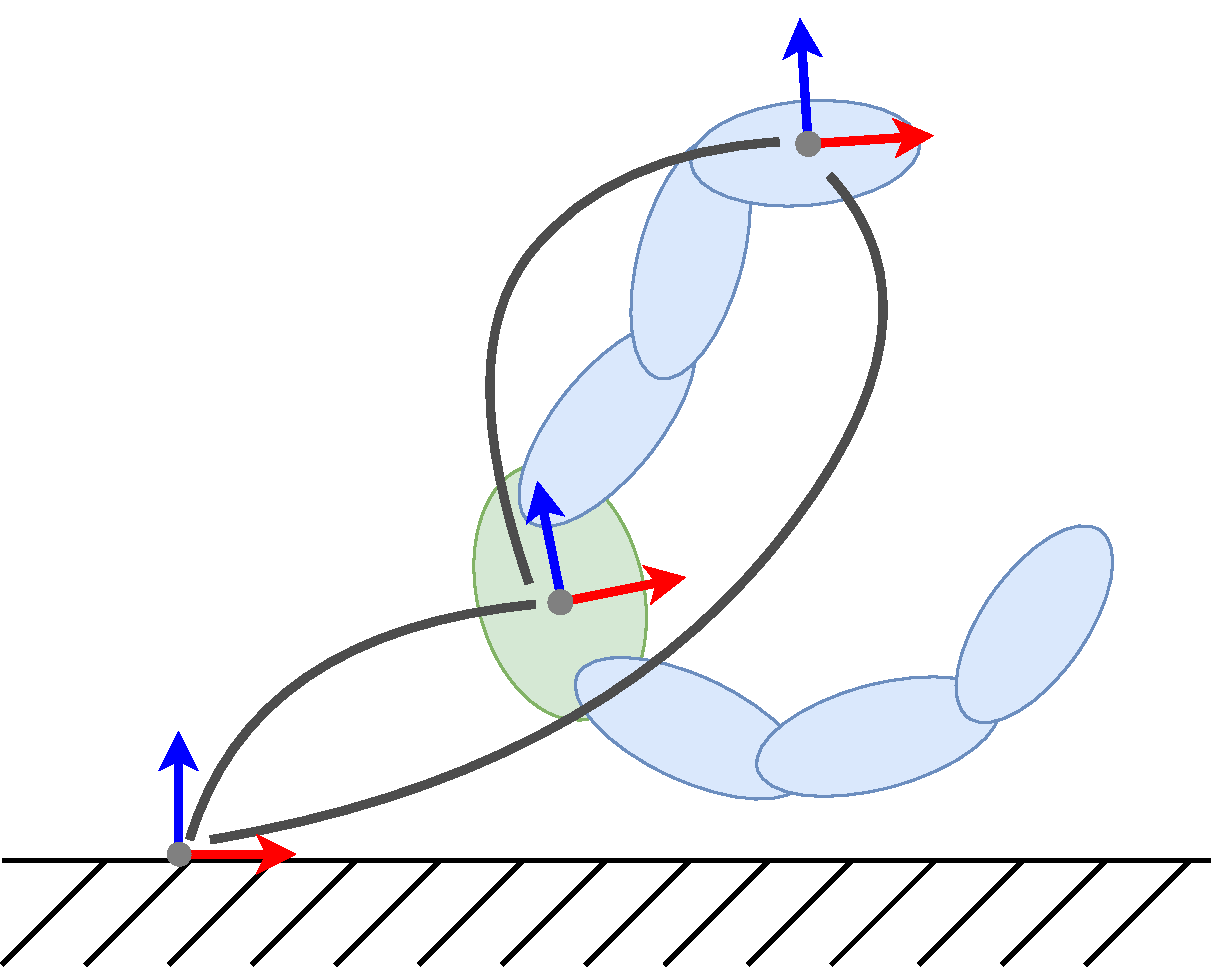
\includegraphics[width=\linewidth]{Figs/forwardKinematics.eps}};
\node[inner sep=0pt] (basePos) at (-4.7,-1.3) {\large $\ls^A H_B$};
\node[inner sep=0pt] (internalPose) at (-1,3) {\large $\ls^B H_L(s)$};
\node[inner sep=0pt] (totalPose) at (4,0) {\large $\ls^A H_L = \ls^A H_B \ls^B H_L(s)$};
\node[inner sep=0pt] (A) at (-4.6,-3) {\Large $A$};
\node[inner sep=0pt] (B) at (-0.5,-1.7) {\Large $B$};
\node[inner sep=0pt] (L) at (2.5,4.3) {\Large $L$};
\end{tikzpicture}
\caption{The pose of a frame $\ls^A H_L$ is a function of the base pose  $\ls^A H_B$ and the shape $s$ of the mechanism.} 
\label{fig:fwdKinematics}
\end{figure}

The velocity of a frame $L$ w.r.t. to the inertial frame is the product between a robot position-dependent Jacobian matrix $J_{L,B/B}(\baseDepVel{B}{q})\in \mathbb{R}^{6\times n+6}$ and the system velocity:
\begin{IEEEeqnarray}{RCL}
\label{eq:velJacobian}
\IEEEyesnumber
\label{velTran}
\ls^L \rmv_{A,L}(\baseDepVel{B}{q},\baseDepVel{B}{\nu}) &=& J_{L,B/B}(\baseDepVel{B}{q}) \nu^B ,\IEEEyessubnumber  \\
\label{eq:linkJacobian}
J_{L,B/B}(\baseDepVel{B}{q}) 
&=& 
\begin{bmatrix}
\ls^{{L}} X_{{B}} &  \ls^L S_{L,B}(\jointPos) 
\end{bmatrix}.\IEEEyessubnumber 
\end{IEEEeqnarray}

The equations~\eqref{homTransf} and \eqref{velTran} represent the so-called \emph{forward kinematics} of the link $L$ using $B$ as the base frame, and using the left-trivialized base velocity, i.e. expressed in the frame $B$. For the time being, in this chapter we will always assume that the base link $B$ is known and fixed, and consequently we will avoid explictly indicating the base dependency on the different quantities, i.e. 
we will simply indicate $q^B$ with $q$, $\nu^B$ with $\nu$, $\ls^L \rmv_{A,L}$ with $\rmv_L$ and $J_{L,B/B}$ with $J_{L/B}$. This assumption will be properly discussed and generalized in Section~\ref{sec:dynamicsWithDiffRepresentation}.

Furthermore, in the next chapter we will discuss how to derive the equation of motions using Lagrangian dynamics. To simplify the notation even more in this section, we will simply assume that we use the left-trivialized representation, i.e. $J_{L/B}$ will be simply indicated $J_L$. Again, this assumption will be properly discussed and generalized in Section~\ref{sec:dynamicsWithDiffRepresentation}.

\subsection{Multibody Lagrangian}

Similarly to the Rigid Body case, for a Multibody system in which the configuration is described by an element of $\SE(3) \times \R^\nDofs$, a generalization of the Euler-Lagrange equations apply, the Hamel equations. In particular the Hamel equations can be seen as a combination of the Euler-Poincare equations for the \emph{base} part, and the classical Euler-Lagrange equation for the joint. 


The Lagrangian for a Free-Floating Mechanical System can be simply obtained as the sum of the Lagrangian of each rigid body.

\begin{IEEEeqnarray}{rCl}
\IEEEyesnumber \label{eq:multiboBodyReducedLagrangian}
    l(q,\nu) &=& k(q,\nu) - U(q) \IEEEyessubnumber \\
    k(q,\nu) &=& \sum_{L \in \mathbb{L}} \ls^L \rmv_{A,L}^T \mathbb{M}_L \ls^L \rmv_{A,L} \IEEEyessubnumber \\
    U(q)     &=& -\sum_{L \in \mathbb{L}} 
    \begin{bmatrix} \ls^A g^T & 0 \end{bmatrix} 
    \ls^A H_L(q) 
    \begin{bmatrix}
    m_L \ls^L c_L \\
    m_L
    \end{bmatrix} \IEEEyessubnumber
\end{IEEEeqnarray}
One major difference between \eqref{eq:rigidBodyReducedLagrangian} and \eqref{eq:multiboBodyReducedLagrangian} is that in \eqref{eq:multiboBodyReducedLagrangian}  the kinematic energy term depends also on the system configuration, rather then just on the velocity.

The following proposition gives us a more convenient form for the left-trivialized lagrangian. 

\begin{proposition}
The left trivialized lagrangian for a multibody defined in \eqref{eq:multiboBodyReducedLagrangian} can be equivalent expressed as: 
\begin{IEEEeqnarray}{rCl}
\label{eq:kinEnergy}
k(q,\nu) &=& \frac{1}{2} \nu^T M(s) \nu \\
U(q) &=& -\begin{bmatrix} \ls^A g^T & 0 \end{bmatrix} 
\ls^A H_B 
\begin{bmatrix}
m \ls^B c(s) \\
m
\end{bmatrix}
\end{IEEEeqnarray}
where $M(s) \in \R^{\nDofs+6 \times \nDofs+6}$ is the system's mass matrix, defined as:
\begin{equation}
M(s) = \sum_{L \in } J_L^T(s) \ls_L \mathbb{M}_L J_L(s), \\
\end{equation}
$m$ is the total mass of the multibody system:
\begin{equation}
m := \sum_{L} m_L
\end{equation}
and $\ls^B c(s)$ is the total center of mass of the multibody system, defined as:
\begin{equation}
\begin{bmatrix}
\ls^B c(s) \\
1
\end{bmatrix}
:= 
\frac{1}{m}
\sum_{L} \ls^B H_L(s) 
\begin{bmatrix}
m_L \ls^L c_L \\
m_L
\end{bmatrix} 
\end{equation}
\end{proposition}

\todo[inline]{provide proof}

The mass matrix has a specific structure, discussed in the next Theorem.

\begin{theorem}[Mass Matrix structure, \citep{wensing2016}]
\label{thm:massMatrixStructure}
The mass matrix $\massMatrix{B}$ can be expressed as follows:
\begin{equation}
\label{eq:massMatrixStructure}
\massMatrix
= 
\begin{bmatrix}
\ls_{B} \bbM(s) & F(s) \\
F^{T}(s) & H(s)
\end{bmatrix},
\end{equation}
with $F_B \in \R^{6 \times n}$ the upper right block of the mass matrix, $H_B \in \R^{n \times n}$ the joint mass matrix and
$\ls_{{B}} \bbM^C$ the so-called \emph{locked 6D rigid body inertia}  of the multi-body system, i.e. 
%the 6D inertia of the robot if it all its joint were \emph{locked} and thus it was a rigid body, i.e. 
\begin{equation}
\ls_{{B}} \bbM(s) = \sum_{L \in \linkSet} \ls_{{B}} X^L(s) \ls_L \bbM_L \ls^L X_{{B}}(s).
 \end{equation}
Furthermore, 
the first six rows of the mass matrix define the jacobian of the articulated body momentum (i.e. the sum of the linear/angular momentum of all the bodies composing the robot), referred to as the \emph{Momentum Matrix}. 
\begin{equation}
\label{eq:momentumMatrix}
{}_{{B}} \rmh =
\begin{bmatrix}
\ls_{{B}} \bbM & F_B
\end{bmatrix} \baseDepVel{B}{\nu} = 
 \sum_{L \in \linkSet} \ls_{{B}} X^L I_L \ls^L \rmv_L.
\end{equation}
\end{theorem}

\begin{remark}
In the following we indicate with $m_L$, $\ls^L c_L$ and $\ls^L \bbM_L$ the \emph{constant} inertial quantities for a specific link $L$. We indicate instead with $m$, $\ls^B c(s)$ and $\ls^L \bbM(s)$ without any subscript the inertial quantities for all the robot. Even if by analogy we use the same symbols we used in describing the dynamics of a single rigid body, always remember that for a multibody this quantities (except for the total mass) are shape-dependent.   
\end{remark}


Plugging this lagrangian in the Hamel equations, we then have that the equations of motions classical form of the equation of a multibody system expressed in the next theorem.
\begin{theorem}
\label{thm:equationsOfMotionForLeftTrivialized}
The equations of motion of a multibody system are given by:
\begin{IEEEeqnarray}{rCl}
\label{eq:equationsOfMotionForLeftTrivialized}
M(s) \dot{\nu} + C(q,\nu) \nu + G(q)
&=&
\begin{bmatrix}
0_{6 \times 1} \\
\tau
\end{bmatrix}
+
\sum_{L \in \mathbb{L}} J_L^T \ls_L \rmf^x  ,
\end{IEEEeqnarray}
where we have:
\begin{IEEEeqnarray}{rCl}
\IEEEyesnumber
M(s) &=& \sum_{L} J_L^T \ls_L \mathbb{M}_L J_L, \IEEEyessubnumber \\
C(q,\nu) &=& \sum_{L} J_L^T \left[ \left( \rmv_L \bar{\times}^* \ls_L \mathbb{M}_L + \ls_L \mathbb{M}_L \rmv_L \times \right) J_L + \ls_L \mathbb{M}_L \dot{J}_L \right],  \IEEEyessubnumber \label{eq:floatingCoriolisMatrixLeftTrivialized} \\
G(q) &=& -M(s) \IEEEyessubnumber
\begin{bmatrix} 
\ls^A R_B^T \ls^A g \\
0_{3 \times 1} \\
0_{\nDofs \times 1} 
\end{bmatrix}. \IEEEyessubnumber
\end{IEEEeqnarray}
\end{theorem}

The proof to this theorem is given in the appendix and in particular in Theorem~\ref{thm:hamelEquations}, as it requires the necessary background in matrix Lie group theory. 

The matrix $C$ is chosen such that the following properties hold on the model~\eqref{eq:equationsOfMotionForLeftTrivialized}:
\begin{proposition}
 \label{massPositiveDef}
 The mass matrix $M$ is symmetric  
 %bounded 
 and positive definite.
 \end{proposition}
\begin{proposition}
 \label{passivity}
The matrix $\dot{M}-2C$ is skew symmetric.
\end{proposition}
\todo[inline]{insert proof}

\begin{remark}
To the best of the authors' knowledge, the compact form of the Coriolis matrix \eqref{eq:floatingCoriolisMatrixLeftTrivialized} was proposed for the first time in \citep{garofalo2013closed}. 
\end{remark}

\begin{remark}
The left-trivialized matrix $M_{B/B}(s)$ depends only on the shape of the system, i.e. it is independent on the base pose $\ls^A H_B$. 
\end{remark}



\todo[inline]{insert proof}

\section{Base Change of Variables}
In the next sections, we will see that the effect of changing base representation and base link choice can be represented as a change of state. We can pose all this transformations as a change of state variables from $(q,\nu)$ to $(\tilde{q},\tilde{\nu})$. Such transformation can model a change of base representation, a change of base link or additional useful system transformation as discussed in Section~\ref{sec:changeBaseAndCentroidal}. An important feature of the class of transformations considered is that they only change how \emph{base} part of the state is represented, while the shape variable representation is assumed to never change. For this reason we will call the following class of transformations \emph{Base Changes of Variables}:

\begin{IEEEeqnarray}{rCl}
\label{eq:stateTransformationStructure}
\tilde{q} &=& (\tilde{H},s) = (H H_T(s), s) \IEEEyessubnumber \\
H_T(s) &\in& \SE(3) \IEEEyessubnumber \\
\tilde{\nu} &=& T(q) \nu , \label{eq:velTransform} \IEEEyessubnumber \\
T(q) &=& 
\begin{bmatrix}
T_{b,b}(q) & T_{b,s}(q) \\
0_{\nDofs \times 6} & 1_{\nDofs}
\end{bmatrix}
\in \R^{(\nDofs + 6) \times (\nDofs + 6)}. \IEEEyessubnumber
\end{IEEEeqnarray}

\begin{assumption}
\label{ass:velTransformIsInvertible}
For each $q$, $T(q)$ is invertible, i.e $$\forall q \in \SE(3) \times \R^\nDofs \hspace{0.5em} \exists \  T^{-1}(q).$$
\end{assumption}
\begin{assumption}
\label{ass:velTransformIsSmooth}
The function $T(\cdot) : \SE(3) \times \R^{\nDofs} \mapsto \R^{6+\nDofs \times 6+\nDofs}$ is smooth.
\end{assumption}
\begin{remark}
Given the triangular structure of $T(q)$, $T(q)$ is invertible if and only if $T_{b,b}(q)$ is invertible. 
\end{remark}
\begin{remark}
The assumption~\ref{ass:velTransformIsInvertible} prevents to use as $T(q)$ a transform that maps base angular velocity to a derivative of a minimal representation of the base orientation, such as Euler Angles, as the resulting transformation would be noninvertible in the singularity point of the representation \citep{stuelpnagel1964}.
\end{remark}

In the next theorem we see how such a transformation affect the multibody dynamics.

\begin{theorem}
\label{thm:baseChange}
Assume that we have a change of variables in the form~\eqref{eq:stateTransformationStructure} that respect Assumption~\ref{ass:velTransformIsInvertible}, that is applied to the system described by the equations of motion introduced in Theorem~\ref{thm:equationsOfMotionForLeftTrivialized}. Then, the following results hold.
\begin{enumerate}
\item The equations of motions~\eqref{eq:equationsOfMotionForLeftTrivialized} transform into
\begin{IEEEeqnarray}{rCl}
\label{eq:reconstructionBaseChange}
\IEEEyesnumber
\dot{\tilde{q}} &=& 
\left( \dot{H}(q,\nu) H_T(s)  + H(q) \dot{H}_T(s,\dot{s})  , \jointVel \right) 
   \IEEEyessubnumber
\\
\label{eq:fb_dynBaseChange}
\tilde{M}(\tilde{q})  \dot{\tilde{\nu}}
&+& \tilde{C}(\tilde{q},\tilde{\nu}) \tilde{\nu}
+ \tilde{G}(\tilde{q}) = 
\begin{bmatrix}
{0}_{6 \times 1} \\
\tau
\end{bmatrix}
+
\sum_{L} \tilde{J}_{L} \rmf_L^{x},
   \IEEEyessubnumber
    \IEEEeqnarraynumspace 
\vspace{-0.15cm}
\end{IEEEeqnarray}
\vspace{-0.15cm}
with (omitting the dependencies to improve readability)
\begin{IEEEeqnarray}{rCl}
\IEEEyesnumber
\label{eq:dynQuantitiesNewBase}
\tilde{M} &=& T^{-T} M T^{-1}  , \IEEEyessubnumber \label{eq:massTrans} \\
\tilde{C} &=&  T^{-T} \left( M \frac{d}{dt}(T^{-1}) +  C T^{-1} \right), \IEEEyessubnumber \label{eq:coriolisTrans} \\
\tilde{G} &=& T^{-T} G .
\IEEEyessubnumber \label{eq:gravityTrans}
\end{IEEEeqnarray}  
\item The free-floating system kinetic energy is given by:
    \begin{IEEEeqnarray}{RCL}
        K = \frac{1}{2} {\tilde{\nu}}^T \tilde{M}(\tilde{q}) \tilde{\nu}  
    \end{IEEEeqnarray}
\item Property~\ref{massPositiveDef} is preserved: if $M$ is symmetric and positive definite then $\tilde{M}$ is symmetric and positive definite.
\item Property~\ref{passivity} is preserved:
if $\dot{M}(q,\nu) - 2 C(q,\nu)$ is skew symmetric, then $\dot{\tilde{M}}(\tilde{q},\tilde{\nu}) - 2 \tilde{C}(\tilde{q},\tilde{\nu})$ is skew symmetric. 
% \item If $T(q)$ is bounded for all $q$, then Property~\ref{} is preserved: the transformed free-floating mass matrix is bounded. 
\end{enumerate}
\end{theorem}
The demonstration of this theorem is given in Subsection~\ref{subsec:proofOfBaseChange}.

This theorem is important because it ensures us that, as long as we transforms the dynamics using a transformation in the form~\eqref{eq:stateTransformationStructure}, for the resulting equations of motion the basic properties required by motion control algorithm holds. Consequently, the control design can choose the representation that he prefers, or in which the specific control synthesis is simplified, without having to verify every time that this properties hold. 

\section{Free Floating Dynamics with different representations or the base velocity}
\label{sec:dynamicsWithDiffRepresentation}
Note that \eqref{eq:equationsOfMotionForLeftTrivialized} presents the equation of motion of the multibody system using the left-trivialized velocity. To obtain the equation of motions for other representations such as the right-trivialized and mixed representation of the multibody velocity, we will just apply some nonlinear transformations for the velocity part of the state. As in this section we need to discuss how to change between different representation of the velocity, we will need to be precise with respect to the representation used, at the expense of the lightness of the notation. Furthermore the equation provided in this section will provide a convenient reference for the rest of the thesis, and for this purpose we need to write them in a non ambiguous way.
In particular, we are interested to understand to which state transformation in the form \ref{eq:stateTransformationStructure} change in base velocity representation from \emph{left-trivialized} to \emph{right-trivialized} or \emph{mixed} representation is associated, to exploit the properties enunciated in the previous section. 

\subsection{Left-trivialized} 
For, we first just rewrite the equations of motion using the complete notation. 

\begin{theorem}
The equations of motions of a multibody system using $B$ as the base link, and using the left-trivialized representation of the base velocity, are given by:
\begin{IEEEeqnarray}{rCl}
\IEEEyesnumber
M_{B/B} (s) \dot{\nu}^{B/B} &+& C_{B/B}(q^B,\nu^{B/B}) \nu^{B/B} + G_{B,B}(q)
= \IEEEnonumber
\\
&=& 
\begin{bmatrix}
0_{6 \times 1} \\
\tau
\end{bmatrix}
+
\sum_{L} J_{L,B/B}^T \ls_L \rmf^x  , \label{eq:eqsMotLT} \IEEEyesnumber
\end{IEEEeqnarray}
where we have:
\begin{IEEEeqnarray}{rCCl}
\IEEEyesnumber
M_{B/B} (s) &=& \sum_{L} J_{L,B/B}^T& \ls_L \mathbb{M}_L J_{L,B/B}, \IEEEyessubnumber \\
C_{B/B}(q^B,\nu^{B/B}) &=& \sum_{L} J_{L,B/B} \Big[& \left( \ls^L \rmv_{A,L} \bar{\times}^* \ls_L \mathbb{M}_L + \ls_L \mathbb{M}_L \ls^L \rmv_{A,L} \times \right) J_{L,B/B} \ + \IEEEnonumber
\\
&&&+ \ls_L \mathbb{M}_L \dot{J}_{L,B/B} \Big],  \IEEEyessubnumber \label{eq:floatingCoriolisMatrixLeftTrivializedCompleteNotation} \\
G_{B/B}(q) &=& M_{B/B}(s)& \IEEEyessubnumber
\begin{bmatrix} 
\ls^A R_B^T \ls^A g \\
0_{3 \times 1} \\
0_{\nDofs \times 1} 
\end{bmatrix}. \IEEEyessubnumber \label{eq:fb_dyn_complete_notation}
\end{IEEEeqnarray}
\end{theorem}

\begin{remark}

Similarly to the rigid body case, the left-hand side of \eqref{eq:eqsMotLT} can be written to depend just on the sensor proper acceleration $\alpha^g_{A,B}$, the body angular velocity $\ls^B \omega_{A,B}$ and the shape position, velocity and accelerations $s, \dot{s}, \ddot{s}$, i.e.:
\begin{IEEEeqnarray}{rCl}
\label{eq:multibodyEqsOfMotWithSensorAcc} 
\IEEEyesnumber
M_{B/B} (s) \dot{\nu}^{B/B} &+& C_{B/B}(q^B,\nu^{B/B}) \nu^{B/B} + G_{B,B}(q)
= \IEEEnonumber
\\
\Gamma(\alpha^g_{A,B},\ls^B \omega_{A,B},s,\dot{s}, \ddot{s})
&=& 
\begin{bmatrix}
0_{6 \times 1} \\
\tau
\end{bmatrix}
+
\sum_{L} J_{L,B/B}^T \ls_L \rmf^x  , \label{eq:eqsMotSensorProper} \IEEEyesnumber
\end{IEEEeqnarray}
Such representation is not convenient when analyzing the multibody system as a dynamical system as it lumps together the linear acceleration of the base with the gravity expressed in body frame, that depends on another part of the state (the rotation between the base frame $B$ and the inertial frame $A$). However, it is extremely convenient in estimation and identification, because $\alpha^G$ and $\ls^B \omega_{A,B}$ can easily be obtained from common inertial sensors, as explained in Chapters~\ref{chap:extForceAndJntTorqueEstimation}~and~\ref{ch:inertialParametersMultiBody}. 
\end{remark}

\subsection{Right-Trivialized}
\begin{lemma}
\label{lem:transformsFromLeftToRight}
Assume that the base velocity representation is changed from \emph{left-trivialized} to \emph{right-trivialized}. Then, the following results hold.
\begin{enumerate}
\item The system position and velocity are subject to the following transformations 
\begin{IEEEeqnarray}{RCL}
\IEEEyesnumber
\label{eq:statetransformationFromLeftToRight}
 H_{T} &=& 1_4, \\ 
\velBaseTrans{B/A}{B/B} &=& 
\begin{bmatrix}
\ls^{A} X_{B} & 0_{6 \times \nDofs} \\
0_{\nDofs \times 6} & 1_{\nDofs}
\end{bmatrix}.
\end{IEEEeqnarray}
\item The jacobian $J_{L,B/A}\in \mathbb{R}^{6\times \nDofs+6}$ of a link frame $L$ is subject to the following transformation
\begin{IEEEeqnarray}{RCL}
\label{eq:jacobianTransFromLeftToRight}
J_{L,B/A} &=& \ls^A X_L J_{L,B/B} \baseTransform{B/B}{B/A}.
\end{IEEEeqnarray}
\end{enumerate}
\end{lemma}

\subsection{Mixed}
\begin{lemma}
\label{lem:transformsFromLeftToMixed}
Assume that the base velocity representation is changed from \emph{left-trivialized} to \emph{mixed}. Then, the following results hold.
\begin{enumerate}
\item The system position and velocity are subject to the following transformations 
\begin{IEEEeqnarray}{RCL}
\IEEEyesnumber
\label{eq:statetransformationFromLeftToMixed}
 H_{T} &=& 1_4 \\ 
\velBaseTrans{B/B[A]}{B/B} &=& 
\begin{bmatrix}
\ls^{B[A]} X_{B} & 0_{6 \times \nDofs} \\
0_{\nDofs \times 6} & 1_{\nDofs}
\end{bmatrix}.
\end{IEEEeqnarray}
\item The Jacobian $J_{L,B/A}\in \mathbb{R}^{6\times \nDofs+6}$ of a link frame $L$ is subject to the following transformation
\begin{IEEEeqnarray}{RCL}
\label{eq:jacobianTransFromLeftToMixed}
J_{L,B/B[A]} &=& \ls^{B[A]} X_L J_{L,B/B} \baseTransform{B/B}{B/B[A]}.
\end{IEEEeqnarray}
\end{enumerate}
\end{lemma}

\section{Free Floating Dynamics with different base links}
Similarly to the change of base velocity representation, also a change of the base link can be represented as \emph{Base Change of Variables}.

The main difference is that a change of base link introduce the transformation matrix $T$ is not block diagonal anymore. Furthermore, the change of variables involves also the base position part of the state, i.e. $H_T \neq 1_4$. To improve the details carried by the complete notation, given a robot velocity $\nu^{B/B}$ and a transformed robot velocity $\nu^{D/D}$ we define $\ls^{D/D} T_{B/B}$ as the matrix for which it holds that:
\begin{equation}
\nu^{D/D} = \ls^{D/D} T_{B/B} \nu^{B/B} . 
\end{equation}
In analogy with the force transformation matrix for $6D$ forces, we also define $\ls_{D/D} T^{B/B}$ as:
\begin{equation}
\label{eq:forceTransform}
\ls_{D/D} T^{B/B} = \left( \ls^{D/D} T_{B/B} \right)^{-T} .
\end{equation}


\begin{property}
The state transformation associated with a change of base link from a link $B$ to a link $D$ is of the form~\ref{eq:stateTransformationStructure}. In particular, it is given, depending on the used velocity representation:
\begin{itemize}
    \item Left-Trivialized Change of Base Link
       \begin{IEEEeqnarray}{rCl}
       H_{T} &=& \ls^B H_D , \\
       \ls^{D/D} T_{B/B} &=& 
       \begin{bmatrix}
         \ls^{{\newBaseFrame}} X_{{B}} & \ls^D S_{\newBaseFrame,B} \\
         0_{\nJoints \times 6} & 1_{\nJoints}
       \end{bmatrix}.
       \end{IEEEeqnarray}
    \item Right-Trivialized Change of Base Link
       \begin{IEEEeqnarray}{rCl}
       H_{\ls^{D/A} T_{B/A}} &=& \ls^B H_D ,\\
       \ls^{D/A} T_{B/A} &=& 
       \begin{bmatrix}
         1_6 & \ls^A S_{\newBaseFrame,B} \\
         0_{\nJoints \times 6} & 1_{\nJoints}
       \end{bmatrix}.
       \end{IEEEeqnarray}
    \item Mixed Change of Base Link
       \begin{IEEEeqnarray}{rCl}
       H_{T} &=& \ls^B H_D , \\
       \ls^{D/D[A]} T_{B/B[A]} &=& 
       \begin{bmatrix}
         \ls^{{\newBaseFrame}[A]} X_{{B}[A]} & \ls^{D[A]} S_{\newBaseFrame,B} \\
         0_{\nJoints \times 6} & 1_{\nJoints}
       \end{bmatrix}.
       \end{IEEEeqnarray}
\end{itemize}

\end{property} 

\begin{remark}[Pure internal joint torques invariance]
Let $\Gamma_{B}$ be a free-floating generalized force acting on the multi-body system. If $\Gamma_{B}$ has a base force-torque equal to zero, then it is independent from the base frame in which it is expressed, i.e.
\begin{equation*}
T^T
 \begin{bmatrix}
0_{6 \times 1} \\
\baseDepTrq{B}{\tau}
\end{bmatrix}
= 
 \begin{bmatrix}
0_{6 \times 1} \\
\baseDepTrq{\newBaseFrame}{\tau}
\end{bmatrix}
=
 \begin{bmatrix}
0_{6 \times 1} \\
\tau
\end{bmatrix}.
\end{equation*}
\end{remark}

\begin{remark}[External joint torque base dependency]
Let assume that $B$ is the base link, and the base dynamics is represented using the left-trivialized representation.
The effect of a pure base force-torque $\ls_B \rmf^x_B$ on a the link $B$ is by definition the generalized force where the first six elements are given by $\rmf^x_B$ and joint part is equal to zero:
$$
\Gamma_{B/B} = 
\begin{bmatrix}
\ls_B \rmf^x_B \\
0_{n\times1} 
\end{bmatrix}.
$$
The generalized force expressed w.r.t. another base link $\newBaseFrame$ is given by:  
\begin{align*}
\Gamma_{\newBaseFrame/D} &= \forceBaseTrans{\newBaseFrame/D}{B/B} \Gamma_{B/B} = 
 \begin{bmatrix}
\ls_{{\newBaseFrame}} X^{{B}} & 0_{6 \times \nJoints} \\
(\ls^D S_{\newBaseFrame,B})^{T} \ls_{{\newBaseFrame}}X^{{B}} & 1_{\nJoints} 
\end{bmatrix} 
\begin{bmatrix}
\rmf^x_B \\
0_{n\times1} 
\end{bmatrix} 
= 
\begin{bmatrix}
\ls_{{\newBaseFrame}} X^{{B}} \ls^B \rmf^x_B \\
(\ls^D S_{\newBaseFrame,B})^{T}  \ls_{{\newBaseFrame}}X^{{B}} \rmf^x_B 
\end{bmatrix} .
\end{align*}
The first six elements of the transformed generalized torques represent the external force-torque $f_B^x$, but expressed with respect to the origin of $D$ rather then the origin of $B$. The last $n$ elements are instead a form of \emph{external joint torques}, and they are non-zero only for the joints on the path from $B$ to $D$. 
It is important to note that contrary to the case of fixed base robots, the \emph{external joint torques} depend on the floating base, and, consequently, they do not describe any meaningful base-invariant physical quantity. 
\end{remark}


\section{System state transformation providing centroidal dynamics}
\label{sec:changeBaseAndCentroidal}

In the humanoid robotics literature, it is widespread to control as primary task the position of the center of mass \citep{ott2011posture} and to minimize the angular momentum of the robot \citep{orin2008centroidal,Orin2013,dai2014whole,herzog2016momentum,Lee2012,koolen2016design}. For analysis purposes, it is then convenient to include the center of mass in the state representing the robot position \citep{ott2011posture,nava2016}.
Such an inclusion can be expressed as a change of variables using the formalism discussed in the previous sections.  Expressing such change of variables in the proposed formalism simplifies the computation of the system dynamics in the new state.

As detailed in the next subsection, the state transformation equations given by using a generic base \emph{frame} rather a base frame rigidly attached to a link are simpler when using the \emph{mixed} representation. Furthermore the works related to multi-task control and centroidal dynamics typically use the \emph{mixed} representation. For this reason in this section we will prefer to use the mixed representation, with the following simplified notation to improve the readability of the section.

\[
  \left[
      \begin{tabular}{@{\quad}m{.05\textwidth}@{\quad}m{.83\textwidth}}
        {\Huge \faInfoCircle} &
          \raggedright%
          \textbf{Simplified Notation, valid for  Section~\ref{sec:changeBaseAndCentroidal}} \par
          \begin{tabular}{@{}p{0.24\textwidth}p{0.55\textwidth}@{}}
               $A$ & Inertial frame. \\
               $\overline{B} := B[A]$ & Frame with the orientation of the inertial frame $A$ and with the origin at the origin of frame $B$.  \\
               $\nu^{C} 
               := 
               \begin{bmatrix}
               \ls^{C[A]} \rmv_{A,C} \\
               s 
               \end{bmatrix}$ & Robot velocity using the mixed velocity of $C$ as the base frame. \\
              $M_{C} 
               := M_{C/C[A]}$ & Mass matrix using $C$ as the base frame and the mixed representation for base quantities. \\
          \end{tabular}
      \end{tabular}
    \right]
\]

\subsection{Frames not rigidly attached to a link}
\label{subsec:framesNotRigidlyAttachedToALink}
So far, the base frame transformation was meant to be between a frame $B$ and a frame $\newBaseFrame$, and both of these frames were assumed to be attached to a physical link. This assumption, however, is not strict. As a matter of fact, we can  assume that the base frame $\newBaseFrame$  is a  frame whose origin is that of a frame $E$, and whose orientation that of a frame $F$: 
\begin{equation}
q^{E[F]} 
:= 
\left( 
\ls^A H_{E[F]}, 
s
\right)
=
\left( 
\begin{bmatrix} 
\ls^A R_F & \ls^A {o}_E \\
0_{3 \times 1} & 0 
\end{bmatrix} 
,  \jointPos  \right).
\end{equation}
Then, the associated generalized robot velocity is given by: 
\begin{equation}
\nu^{E[F]} = 
\begin{bmatrix}
\ls^A \dot{o}_E \\
\ls^A \omega_{A,F} \\ 
\jointVel
\end{bmatrix} 
= 
\begin{bmatrix}
\ls^A \dot{o}_E \\
 \left(\ls^A\dot{R}_{F} \ls^A {R}_{F}^{T} \right)^\vee \\ 
\jointVel
\end{bmatrix} 
\end{equation}

The new \emph{base} velocity reflect the different choices of the \emph{base} position variables. The Jacobian of the velocity of a frame defined in such a compound way 
%assuming a floating base $\newBaseFrame$ 
is simply given by the combination of the linear part (first three rows) of $J_{C,B}$, indicated with $J_{C,B}^l \in \R^{3 \times (6+n)}$ and the angular part of (last three rows) of $J_{D,B}$, indicated with $J_{D,B}^a \in \R^{3 \times (6+n)}$: 
\begin{equation}
\label{eq:compoundFrameVelocity}
J_{E[F],B} = 
\begin{bmatrix} 
J_{E,B}^l \\
J_{F,B}^a
\end{bmatrix}.
\end{equation}
Note that the property of \eqref{eq:compoundFrameVelocity} be the simple stacking of the linear and angular Jacobians is a consequence of the use of \emph{mixed} velocity representation.  Indeed the equivalent jacobians using the \emph{inertial} or \emph{body-fixed} representation are related in a more complex way to the Jacobians of frame $E$ and $F$.

From \eqref{eq:compoundFrameVelocity}, one obtains the transformation matrix $\ls^{E[F]} T_{B}$ to be used in a base variable changed defined as in :
\begin{equation}
H_T = \ls^B H_{E[F]} \\ 
\ls^{E[F]} T_{B} =
\begin{bmatrix}
\multicolumn{2}{c}{J_{E[F],B}} & \\
0_{6 \times n} & 1_{n \times n} 
\end{bmatrix}.
\end{equation}


\subsection{Recalls on centroidal dynamics quantities}
To properly define the \emph{centroidal dynamics}, it is convenient to define a frame $\overline{G}$ whose origin is the center of mass of the multi body system, and whose orientation is that of the inertial frame $A$.
Note that the use of $\overline{G}$ is an abuse of notation, as we \emph{do not} define an orientation for frame $G$ (see Figure~\ref{fig:centroidalFigure}).

Then, the total  momentum and the composite rigid body inertia (CRBA) of the system expressed w.r.t. the $\overline{G}$ frame are given by: 
\begin{align}
\label{eq:centroidalMomentum}
\ls_{\overline{G}} \rmh = \ls_{\overline{G}} X^{\overline{B}} \ls_{\overline{B}} \rmh, && \ls_{\overline{G}} I^C = \ls_{\overline{G}} X^{\overline{B}} \ls_{\overline{B}} I^C  \ls^{\overline{B}} X_{\overline{G}}.
\end{align}
In the robotics literature, these quantities are known as  \emph{Centroidal Momentum} and as \emph{Centroidal Composite Rigid Body Inertia (CCRBI)}  \citep{Orin2013}, respectively.
The structure of these \emph{centroidal} quantities is the following \citep{Orin2013} :
\begin{align}
\label{eq:centroidalMomentumStructure}
\ls_{\overline{G}} \rmh = 
\begin{bmatrix}
m \ls^A \dot{c} \\
\ls_{\overline{G}} \rmh^a
\end{bmatrix},
&& 
\ls_{\overline{G}} I^C = 
\begin{bmatrix}
m 1_{3\times3} & 0_{3\times3} \\
0_{3\times3}   & L^C
\end{bmatrix},
\end{align}
with $m \in \R$ the total mass of the robot, $\ls^A c \in \R^3$ the center of the mass of the robot expressed in the inertial frame, $\ls_{\overline{G}} \rmh^a \in \R^3$ the total angular momentum and $L^C \in \R^{3\times3}$ the locked 3D inertia of the robot , both expressed in $\overline{G}$.

Given a base frame $B$, note that the matrix $A_{G,B} \in \R^{6 \times (n+6)}$ that multiplied by the generalized robot velocities vector $\nu^B$ gives the \emph{centroidal momentum} can be easily obtained from the floating base mass matrix.
In fact, by combining \eqref{eq:momentumMatrix} and \eqref{eq:centroidalMomentum} one has:
\begin{IEEEeqnarray}{rClrCl}
\label{eq:centroidalMomentumMatrix}
\ls_{\overline{G}} \rmh = A_{G,B} \nu^B ,
\quad
 A_{G,B} &=& 
\ls_{\overline{G}} X^{\overline{B}}
\begin{bmatrix}
\ls_{\overline{B}} I^C & F_B
\end{bmatrix}.
\end{IEEEeqnarray}

The $A_{G,B}$ matrix is known as the \emph{Centroidal Momentum Matrix} \citep{orin2008centroidal,Orin2013}.

\subsection{Average 6D Velocity}
\label{subsec:avgSixDVel}

In the humanoids whole-body control literature, it is common to define the \emph{average 6D velocity} $\rmv_G$  of the robot as \citep{Orin2013}: 
\begin{align}
\label{eq:averageVelocity}
\rmv_G =  (\ls_{\overline{G}} I^C)^{-1} \ls_{\overline{G}} \rmh = 
\begin{bmatrix}
\frac{1}{m} (m \ls^A \dot{o}_G) \\
(L^C)^{-1} \ls_{\overline{G}} \rmh^a
\end{bmatrix} 
=
\begin{bmatrix}
 \ls^A \dot{o}_G \\
\omega_G 
\end{bmatrix}.
\end{align}

By definition, the linear part of the  \emph{average 6D velocity} (i.e. the first three components of $\rmv_G$) is simply the velocity of the center of mass of the system. Its angular part (i.e. the last three components) is called 
the \emph{average angular velocity}  $\omega_G$  \citep{jellinek1989separation,Essen2004,morita2003attitude}, even if this name is an abuse of the term \emph{angular velocity} because $\omega_G$ is not defined as the angular velocity of an orientation frame. 
In fact, a rotation matrix $R(\jointPos) \in SO(3)$ such that $R(\jointPos)R^{T}(\jointPos) = \omega_G^{\wedge}$ exists only for a limited class of multibody systems \citep{saccon2017}. 
The \emph{average angular velocity} has a precise physical meaning if a multibody system is evolving without external forces acting on it. If a generalized impulse blocks all its joint motions instantaneously, the resulting rigid body would evolve with an angular velocity $\omega_G$. For this reason, $\omega_G$ is also known as the \emph{locked angular velocity} in geometrical mechanics literature \citep{marsden1993reduced}. 

The relationship between the generalized robot velocities vector $\nu^B$ and the \emph{centroidal velocity} $\rmv_G$ can be easily obtained by combining \eqref{eq:centroidalMomentumMatrix} and \eqref{eq:averageVelocity}:
\begin{IEEEeqnarray*}{rCl}
\rmv^G &=& {(\ls_{\overline{G}} I^C)}^{-1} A_{G,B} \nu^B = 
{(\ls_{\overline{G}} I^C)}^{-1} \ls_{\overline{G}} X^{\overline{B}}
\begin{bmatrix}
\ls_{\overline{B}} I^C & F_B
\end{bmatrix} \nu^B = \\
&=& 
\begin{bmatrix}
\ls^{\overline{G}} X_{\overline{B}} & 
{(\ls_{\overline{G}} I^C)}^{-1} \ls_{\overline{G}} X^{\overline{B}} F_B
\end{bmatrix} \nu^B .
\end{IEEEeqnarray*}
Noting that this matrix has the same structure of the  floating base jacobian \eqref{eq:linkJacobian}, we borrow the notation we use for the Jacobians of links, even if $\rmv_G$ is not defined as the mixed velocity of a well defined frame. So, we define $J_{G,B}$ and $S_{G,B}$ such that:
\begin{equation}
\nu^G = J_{G,B} \nu^B ,
\end{equation}
\begin{equation}
\label{eq:centroidalVelJacobian}
J_{G,B} :=
\begin{bmatrix}
\ls^{\overline{G}} X_{\overline{B}} & \hspace{1em} 
S_{G,B} 
\end{bmatrix}
:= 
\begin{bmatrix}
\ls^{\overline{G}} X_{\overline{B}} & \hspace{1em} 
(\ls_{\overline{G}} I^C)^{-1} \ls_{\overline{G}} X^{\overline{B}} F_B
\end{bmatrix}.
\end{equation}

\subsection{Centroidal change of variables}
\subsubsection{Including the center of mass in the robot state}
For the sake of including the center of mass in the multibody dynamics, we can define a new robot position as follows:
\begin{equation}
\robotPos^{G[B]} = (\ls^{\inertialFrame}c ,\ls^{\inertialFrame}R_{\bodyFrame},\jointPos) .
\end{equation}
This implies that:
\begin{equation}
\nu^{G[B]} 
= 
\begin{bmatrix}
 \multirow{2}{*}{$\rmv_{G[B]}$}\\
  \\
 \jointVel 
\end{bmatrix}
= 
\begin{bmatrix}
 \ls^{\inertialFrame}\dot{c} \\
 (\ls^{\inertialFrame}\dot{R}_{\bodyFrame} \ls^{\inertialFrame}{R}_{\bodyFrame}^{T})^\vee \\ 
 \jointVel 
\end{bmatrix}.
\end{equation}

The corresponding transformation matrix is given by, as explained in subsection~\ref{subsec:framesNotRigidlyAttachedToALink}: 
\begin{equation}
\ls^{G[B]} T_{B} = 
\begin{bmatrix}
\multicolumn{2}{c}{J^l_{G[B],B}} &  \\ 
0_{3 \times (3+n)} & 1_{(3+n) \times (3+n)}  
\end{bmatrix},
\end{equation}
where $J^l_{G[B],B}$ is the center of mass jacobian, i.e. the matrix such that 
\[\ls^A \dot{c} = J^l_{G[B],B} \nu_B.\]
Note that this is also equal to the first three rows of \eqref{eq:centroidalVelJacobian}, i.e. $J^l_{G[B],B} = J^l_{G,B}$.
The change of base introduced by $\ls^{G[B]} T_B$ is the one used in \citep{ott2011posture}.

\begin{figure}
\begin{tikzpicture}
\node[inner sep=0pt] (floatingBase) at (0,0) {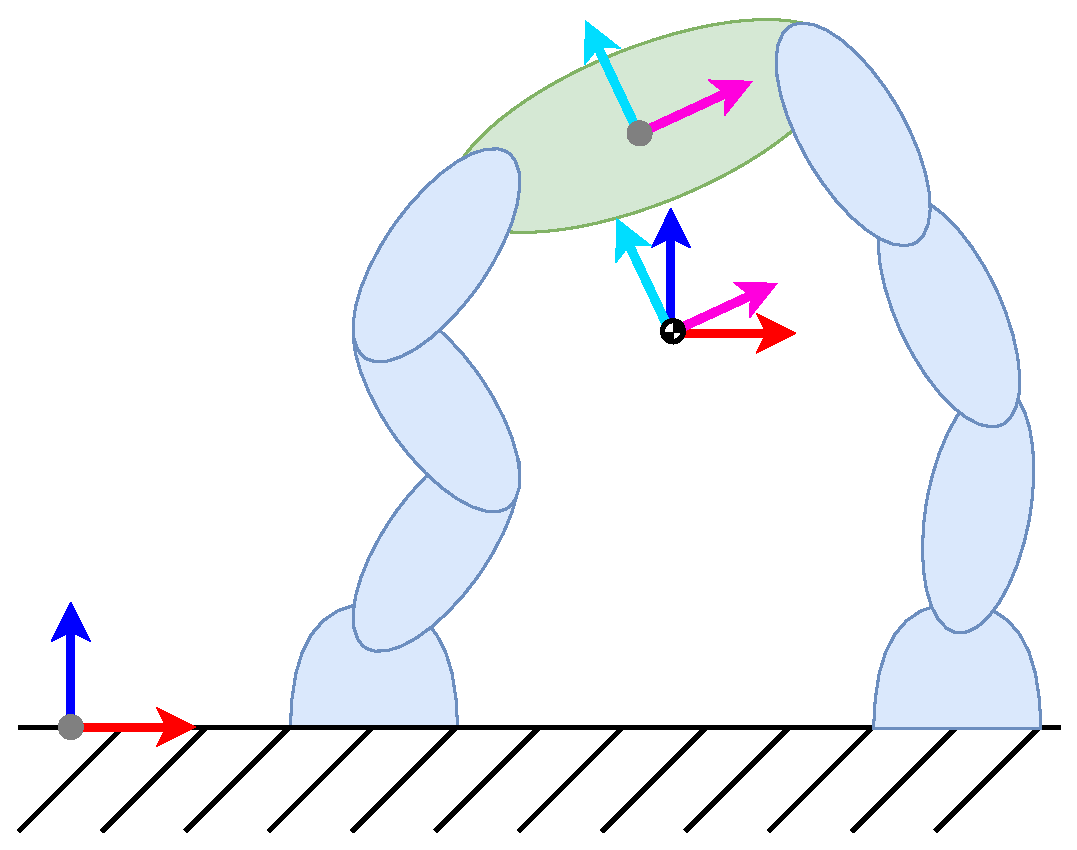
\includegraphics[width=\linewidth]{Figs/COMFrames.eps}};
\node[inner sep=0pt] (A) at (-5,-3.3) {\Large $A$};
\node[inner sep=0pt] (B) at (0.5,3.2) {\Large $B$};
\node[inner sep=0pt] (GrotB) at (0.5,1.2) {\Large $G[B]$};
\node[inner sep=0pt] (GrotA) at (2.3,0.3) {\Large $G[A]$};
\end{tikzpicture}
\caption{Graphical depiction of frames $A$, $B$, $G[A]$ and $G[B]$ for an example two legged robot.}
\label{fig:centroidalFigure}
\end{figure}

\subsubsection{Block diagonalization of the mass matrix}
Using the definition of \emph{average 6D velocity} of the multibody system, we can define a \emph{centroidal} generalized joint velocities vector in which we combine the average 6D velocity and the joint velocities :
\begin{equation}
\nu^G 
= 
\begin{bmatrix}
 \rmv_G \\
 \jointVel 
\end{bmatrix}.
\end{equation}
Let us remark (again) that there is no such thing as a $G$ frame: the notation $\nu^G$ is an abuse of notation. In particular, it does not make sense to write $q^G$ : the change of variables induced by the use of the average 6D velocity is only a change of variables in the velocity space, while for the position space it is usually convenient to continue to use the $q^{G[B]}$ position introduced before.

The mapping $\ls^G T_B$ from the \emph{floating base} generalized velocities $\nu^B$ to $\nu^G$ has the same structure of the change of variables introduced in \eqref{eq:velTransform}: 
\begin{IEEEeqnarray}{rClrCl}
\label{eq:centrTransform}
\nu^G 
&=&
\ls^G T_B \nu^B , \quad 
\ls^G T_B
=
\begin{bmatrix}
\ls^{\overline{G}} X_{\overline{B}} & S_{G,B} \\
0_{\nJoints \times 6} & 1_{\nJoints \times \nJoints}
\end{bmatrix} .
\end{IEEEeqnarray}
This induces a change of variables also on the generalized robot forces, as detailed in \eqref{eq:forceTransform}, i.e. : 
\begin{equation}
\IEEEyesnumber
\label{eq:centrTransformForce}
\ls_G T^B =
\ls^G T_B^{-T} = 
\begin{bmatrix}
\ls_{\overline{G}} X^{\overline{B}} & 0_{6 \times \nJoints} \\
-S_{G,B}^{T} \ls_{\overline{G}} X^{\overline{B}} & 1_{\nJoints}
\end{bmatrix}.
\end{equation}
Using the transformation $\ls^G T_{B}$ in \eqref{eq:dynQuantitiesNewBase}, one can obtain the equations of motion with $(q^{G[B]},\nu^G)$ as state, i.e. : 
\begin{IEEEeqnarray}{rCl}
\IEEEyesnumber
\dot{q}^{G[B]} &=&
\left(  
 \begin{bmatrix} 
 \ls^A \omega_{A,B}^{\wedge}(\nu^G) \ls^A R_B
 & \ls^A\dot{c} \\
 0_{3\times1} & 0 
 \end{bmatrix}
 ,\jointVel \right) , \IEEEyessubnumber \label{eq:centroidalReconstruction} \\
\massMatrix{G}(q^{G[B]})  \robotAcc{G}
&+& C_{G}(q^{G[B]},\robotVel{G}) \robotVel{G}
+ \gravityTrq{G} =
\begin{bmatrix}
{0}_{6 \times 1} \\
\tau
\end{bmatrix}
+
\sum_{L \in \mathfrak{L}} J_{L,G}^{T} \rmf_L^{x},
   \IEEEyessubnumber \label{eq:fb_dyn_centroidal}
    \IEEEeqnarraynumspace 
\end{IEEEeqnarray}
where $\ls^A \omega_{A,B}(\nu^G)$ is the angular velocity of the link $B$ as a function of the \emph{centroidal} generalized joint velocity $\nu_G$. 

The equations of motion \eqref{eq:fb_dyn_centroidal} incorporate in the first six rows what is usually called the \emph{centroidal dynamics}, together with the joint dynamics in a single set of equations of motions. 
The specific features of such a representation of the equations of motion are highlighted in the following theorem, and they have been already exploited in \citep{nava2016}. 
\begin{lemma}
\label{lem:centroidalDynamics}
For the equations of motion given by \eqref{eq:fb_dyn_centroidal}, the following results hold.
\begin{enumerate}
\item The (centroidal) mass matrix $M_G$ has a block 
diagonal structure, i.e. :
\begin{equation}
\label{eq:centroidalMassMatrix}
M_G(q^{G[B]}) = 
\begin{bmatrix}
m 1_{3} & 0_{3\times3} & 0_{3\times \nJoints} \\
0_{3\times3} & L^C(q^{G[B]}) & 0_{3\times \nJoints} \\
0_{3\times3} & 0_{3\times3} & H_G(s)
\end{bmatrix} 
\end{equation}
where $m \in \R$ is the total mass of the system, $L^C \in \R^{3 \times 3}$ is the \emph{locked} 3D inertia matrix of the system expressed in the center of mass and with the orientation of the absolute frame $A$ and $H_G(s) \in \R^{n \times n}$ is the centroidal joint mass matrix.

\item The (centroidal) gravity term $G_G$ is independent from the robot state and has the following structure: 
\begin{equation}
G_G = 
\begin{bmatrix}
-m \ls^Ag \\
0_{3\times1} \\
0_{\nJoints\times1}
\end{bmatrix}
\end{equation}
where $\ls^Ag \in \R^3$ is the gravitational acceleration expressed in the frame $A$.

\item Assuming that Property~\ref{passivity} holds for $M_B$ and $C_B$, the (centroidal) coriolis matrix $C_G$ has a block diagonal structure, i.e. :
\begin{equation}
C_G(q^{G[B]},\nu^G) = 
\begin{bmatrix}
0_{3\times3} & 0_{3 \times (n+3)} \\
0_{3 \times (n+3)} & C^{\text{aj}}_G(q^{G[B]},\nu^G) 
\end{bmatrix}
\end{equation}
where $C^{\text{aj}}_G(q^{G[B]},\nu^G) \in \R^{(3+n)\times(3+n)}$ is the centroidal coriolis matrix for the angular and joint part of the dynamics.
\end{enumerate}
\end{lemma}

The proof for Lemma~\ref{lem:centroidalDynamics} is provided in Subsection~\ref{proof:centroidalDynamics}.

\section{Proofs}
\subsection{Proof of Theorem~\ref{thm:baseChange}}
\label{subsec:proofOfBaseChange}
\begin{enumerate}
    \item First, notice that the time derivative of  \eqref{eq:velTransform} yields:
\begin{equation}
\label{eq:accTrans}
\dot{\tilde{\nu}}
= 
T \dot{\nu}
+ 
\dot{T}
{\nu} .
\end{equation}
Then, the equations of motion \eqref{eq:fb_dynBaseChange} can be obtained by substituting $\dot{\nu}$ obtained from \eqref{eq:accTrans} into \eqref{eq:equationsOfMotionForLeftTrivialized}, by substituting $\nu$ obtained from \eqref{eq:velTransform} into \eqref{eq:equationsOfMotionForLeftTrivialized} and by multiplying the obtained equation times $T^{-T}$.
    \item In view of \eqref{eq:kinEnergy}, i.e.:
    \begin{equation*}
        k = \frac{1}{2} {\nu}^T M(q)  \nu , 
    \end{equation*}
    and of $\tilde{\nu} =  T \nu$ one has : 
    \begin{equation*}
    k = \frac{1}{2} \tilde{\nu}^T T^{-T} M T^{-1} \tilde{\nu} . 
    \end{equation*}
    From which we obtain that the kinematic energy is also given by:
    \begin{IEEEeqnarray*}{rClrCl}
    k  &=& \frac{1}{2} \tilde{\nu}^T \tilde{M} \tilde{\nu}, \quad
        \tilde{M} &=& T^{-T} M T^{-1} .
    \end{IEEEeqnarray*}
    \item The simmetry and positive definiteness of $\tilde{M}$ follow from the expression of the kinetic energy given in the previous step.
    \item The condition that $\dot{M} -  2C$ is skew-symmetric is equivalent to the condition that
$\dot{M} = C + C^{T} $. So, we will demonstrate that $\dot{M} - C - C^{T} = 0_{(n+6) \times (n+6)}$ implies $\dot{\tilde{M}} - \tilde{C} - \tilde{C}^{T} = 
0_{(n+6) \times (n+6)}$.
Let us write  $\dot{\tilde{M}} - \tilde{C} - \tilde{C}^{T}$ using \eqref{eq:massTrans} and 
\eqref{eq:coriolisTrans}, i.e. :
\begin{eqnarray*}
\dot{\tilde{M}} - \tilde{C} - \tilde{C}^{T} = \\
=
\underbrace{
\frac{d}{dt} \left( {T}^{-T} \right) M T^{-1}  +
T^{-T} \dot{M} T^{-1} + 
T^{-T} M  \frac{d}{dt} \left( T^{-1} \right)}_{\dot{\tilde{M}}} \\  
 \underbrace{- T^{-T} M \frac{d}{dt} \left( T^{-1} \right)  - T^{-T} C  T^{-1}}_{ -\tilde{C} } \\  
 \underbrace{- \frac{d}{dt} \left( T^{-T}\right)  M  T^{-1} -  T^{-T} {C}^T  T^{-1} }_{ -\tilde{C}^T }
 \end{eqnarray*}
We can then write:
\begin{eqnarray*}
\dot{\tilde{M}} - \tilde{C} - \tilde{C}^{T} = \\
 T^{-T} \left( \dot{M} - C - C^{T} \right) T^{-1} + \\
 + \frac{d}{dt} \left( {T}^{-T} \right) M T^{-1}  - \frac{d}{dt} \left( {T}^{-T} \right) M T^{-1}  + \\ + T^T M  \frac{d}{dt} \left( T^{-1} \right) - T^T M  \frac{d}{dt} \left( T^{-1} \right)
\end{eqnarray*}
 Using the hypothesis that $\dot{M} - C - C^{T} = 0_{(n+6) \times (n+6)}$ we can then conclude that $\dot{\tilde{M}} - \tilde{C} - \tilde{C}^{T} = 0_{(n+6) \times (n+6)}$.

\end{enumerate}
$\hfill\blacksquare$

\subsection{Proof of Lemma~\ref{lem:centroidalDynamics}}
\label{proof:centroidalDynamics}

\begin{enumerate}
\item The \emph{centroidal} mass matrix can be obtained by applying \eqref{eq:centrTransform} to~\eqref{eq:dynQuantitiesNewBase}, i.e. :
\begin{equation}
M_G = \ls_G T^B M_B \ls^B T_G .
\end{equation}
By exploiting the structure  of $M_B$ and $\ls_G T^B$ in  \eqref{eq:massMatrixStructure} and \eqref{eq:centrTransformForce}, and recalling that $\ls_{\overline{G}} X^{\overline{B}} = \ls^{\overline{B}} X_{\overline{G}}^T$ one has:
\begin{IEEEeqnarray}{rCl}
\IEEEyesnumber
M_G &=& 
\begin{bmatrix}
\ls_{\overline{G}} X^{\overline{B}} & 0_{6 \times \nJoints} \\
S_{B,G}^T & 1_{\nJoints \times \nJoints}
\end{bmatrix}
\begin{bmatrix}
\ls_{\overline{B}} I^C & F_B \\
F_B^T & H_B 
\end{bmatrix}
\begin{bmatrix}
\ls^{\overline{B}} X_{\overline{G}} & S_{B,G} \\
0_{6 \times \nJoints} & 1_{\nJoints \times \nJoints}
\end{bmatrix} = \IEEEyessubnumber
 \\
&=&
\begin{bmatrix} 
\ls_{\overline{G}} X^{\overline{B}} \ls_{\overline{B}} I^C \ls^{\overline{B}} X_{\overline{G}} 
&
\ls_{\overline{G}} X^{\overline{B}} \left( \ls_{\overline{B}} I^C S_{B,G} +  F_B \right)
\\
\left( S_{B,G}^T \ls_{\overline{B}} I^C + F_B^T \right) \ls^{\overline{B}}  X_{\overline{G}} 
&
H_G
\end{bmatrix} \IEEEyessubnumber \label{eq:centroidalMassMatrixWithExplicitOffDiagonalTerms}
\end{IEEEeqnarray}
with $H_G = S_{B,G}^T \ls_{\overline{B}} I^C S_{B,G} +
S_{B,G}^T F_B + F_B^T S_{B,G} +
H_B$ .

In view of \eqref{eq:centroidalMomentum} and \eqref{eq:centroidalMomentumStructure}, then $\ls_{\overline{G}} X^{\overline{B}} \ls_{\overline{B}} I^C \ls^{\overline{B}}X_{\overline{G}}$ can be written as the \emph{centroidal composite rigid body inertia}, i.e. : 
\begin{equation}
\label{eq:centroidalMassMatrixComputations}
\ls_{\overline{G}} X^{\overline{B}} \ls_{\overline{B}} I^C \ls^{\overline{B}} X_{\overline{G}} = \ls_{\overline{G}} I^C = \begin{bmatrix}
m 1_{3\times3} & 0_{3\times3} \\
0_{3\times3}   & L^C
\end{bmatrix}.
\end{equation}
Using \eqref{eq:centroidalVelJacobian}, it is possible to write $S_{B,G}$ as:
\begin{equation}
\label{eq:centroidalJointJacobian}
S_{B,G} = - {\ls}^{\overline{B}} X_{\overline{G}} S_{G,B} = 
- \left( \ls_{\overline{B}} I^{C} \right)^{-1} F_B . 
\end{equation}
Substituting \eqref{eq:centroidalJointJacobian} in the off-diagonal terms of 
\eqref{eq:centroidalMassMatrixWithExplicitOffDiagonalTerms} it is possible to show that the off-diagonal terms are equal to $0_{6 \times n}$. 

\item Exploiting the gravity generalized forces structure given by \eqref{eq:gravityTrans} and the structure of $M_G$ given in \eqref{eq:centroidalMassMatrix}, we can write $G_G$ as:
$$
G_G = - M_G \begin{bmatrix} \ls^A g \\ 0_{3 \times 1}  \\ 0_{n \times 1}  \end{bmatrix} = \begin{bmatrix} - m \ls^A g \\ 0_{3 \times 1}  \\ 0_{n \times 1}  \end{bmatrix} .
$$

\item From the structure of the centroidal dynamics \eqref{eq:fb_dyn_centroidal}, and from the Newton equation $m \ls^A\ddot{c} - m \ls^Ag = \sum_{L \in \mathfrak{L}} \ls^A f^x_L$ we have that the $C_G$ matrix has the following structure:
\begin{equation}
\label{eq:preliminaryCentroidalCoriolisSparsity}
\begin{bmatrix}
0_{3 \times 3} & 0_{3 \times (n+3)} \\
C_{G}^{\text{offDiag}} & C^{\text{aj}}_G \\ 
\end{bmatrix}.
\end{equation}

From the assumption given by Property~\ref{passivity} that $(\dot{M}_B - 2C_B)^T = (2C_B - M_B)$ by applying Theorem~\ref{thm:baseChange} we obtain that:
\begin{equation} 
\label{eq:centroidalPassivity}
C_G + C_G^T = \frac{\dot{M}_G}{2} .
\end{equation}
Plugging the the sparsity patterns \eqref{eq:preliminaryCentroidalCoriolisSparsity} and \eqref{eq:centroidalMassMatrix} in the \eqref{eq:centroidalPassivity}, extracting the top left $3 \times n$ subblock one obtains that:
$$
  0_{3 \times (n+3)} + \left( C_{G}^{\text{offDiag}} \right)^T = 0_{3 \times (n+3)}
$$
from which: 
$$
C_{G}^{\text{offDiag}} = 0_{(n+3) \times 3}.
$$
\end{enumerate}
$\hfill\blacksquare$
